\documentclass[aps,pra,twocolumn,superscriptaddress,longbibliography,floatfix,nofootinbib]{revtex4-2}

\usepackage{amsmath,amssymb}
\usepackage{graphicx}
\usepackage{hyperref}
\usepackage{braket}

\hypersetup{
  colorlinks=true,
  linkcolor=blue,
  citecolor=blue,
  urlcolor=blue,
  pdftitle={CHSH-Form Values Above 2 in Fibonacci Anyon Braiding: A
  Complete Landscape of Braid Words up to Length 12},
  pdfauthor={Berkay Y{\"u}ksel Sayim},
  pdfsubject={quant-ph; Fibonacci anyons; CHSH inequality; topological quantum computation},
  pdfkeywords={Fibonacci anyons, CHSH inequality, braiding landscape,
  entanglement, measurement protocol, non-Abelian anyons, autocorrelation}
}

\begin{document}

\setcounter{secnumdepth}{3}

\title{CHSH-Form Values Above 2 in Fibonacci Anyon Braiding:\\ A
Complete Landscape of Braid Words up to Length 12}

\author{Berkay Y\"uksel Sayim}
\email{berksa@tutamail.com}
\affiliation{Independent Research, Germany}
\affiliation{\href{https://orcid.org/0009-0004-4993-7352}{ORCID: 0009-0004-4993-7352}}

\date{2026-10-03}

\begin{abstract}
We report a complete sequence-by-sequence landscape of CHSH-form values
for six Fibonacci anyons in two encodings, covering all words of length
$L=3$--$12$ with two generators and $L=2$--$9$ with three. In the
two-generator $d_{1b}$ encoding, braiding alone cannot exceed the
classical value: the two generators act on different anyons and commute,
and all $8190$ braid words of length $L=1$--$12$ give $|S|=2$ exactly on
the leakage-free fusion code. A two-qubit circuit built from the same
Fibonacci $F$- and $R$-matrices, which does not satisfy the braid
relations, reaches $|S|=2.733$ at $L=12$ with the standard Fibonacci
data ($96.6\%$ of the Tsirelson bound $2\sqrt{2}$) and $|S|=2.811$ at
the optimum over a phase deformation; this excess is therefore not a
braiding effect. Throughout, ``CHSH violation'' denotes a CHSH value
exceeding~2 on the Fibonacci fusion space, which does not factorize into
spatially separated Alice/Bob subsystems; the reported values are
signatures of nonseparability and single-algebra contextuality, not Bell
violations in the Einstein--Podolsky--Rosen sense. In the
three-generator encoding, the generator~$\sigma_3$ that acts across the
bipartition is the only source of entanglement: without it, the state
stays in the fusion code as a product state, for all sequences and
deformation phases. Under four-dimensional computational-subspace
projection the maximum is $|S|=2.824$ at $L=8$, and $91.8\%$ of the
words exceed 2 at $L=9$, including $510$ words without $\sigma_3$ that
do so only through the projection; a Horodecki-type score on the native
five-dimensional observables exceeds 2 for $42.8\%$. Sequential braiding
on a shared fusion space produces a positive lag-1 autocorrelation of
the simulated CHSH value, $\text{ACF}(1)=+0.35$ at $11.22\sigma$, because the
state is carried from step to step; a null test with
independently drawn phases shows none.
\end{abstract}

\keywords{Fibonacci anyons, CHSH inequality, braiding landscape,
entanglement, measurement protocol,
non-Abelian anyons, autocorrelation}

\maketitle



%% ====================================================================
%%  SECTION 1 — INTRODUCTION
%% ====================================================================
\section{Introduction}
\label{sec:intro}

Non-Abelian anyons in two-dimensional topological phases support
braiding operations that can generate entanglement between logical
qubits encoded in the fusion space~\cite{Nayak2008,Freedman2003}.
For Fibonacci anyons---the simplest non-Abelian species with a
universal gate set---explicit braiding sequences implementing quantum
gates have been compiled~\cite{Bonesteel2005,Hormozi2007}, and
CHSH-violating settings on the Fibonacci fusion space have been
constructed~\cite{Brennen2009}.
However, a basic question has remained open:
\emph{what fraction of all possible braiding sequences produces
CHSH violation, and what controls the boundary between violating
and nonviolating sequences?}

We address this question by exhaustive enumeration.
For six Fibonacci anyons on a linear fusion tree, we compute the
maximal CHSH value $|S|$ for every braiding sequence in two
distinct encodings: a two-generator encoding
($d_{1b}$, $L=3$--$12$, native four-dimensional Hilbert space)
and a three-generator encoding ($L=2$--$8$ fully enumerated, $L=9$ for
CHSH-fraction statistics, and the $\delta = 0$ maxima over all $3^L$ words at
$L = 10$ and $12$; full five-dimensional fusion space).
Throughout, the two-generator case is enumerated in its
\emph{circuit model}: a pair of two-qubit gates built from the
Fibonacci $F$- and $R$-matrices, which do not satisfy the braid
relations. We distinguish it from the $d_{1b}$ \emph{fusion code},
the leakage-free five-dimensional realization of the same encoding,
in which both generators act strictly locally. Every $|S|$ value
reported for $d_{1b}$ below refers to the circuit model.
The enumeration comprises $2^L$ sequences in $d_{1b}$ and $3^L$
sequences in the three-generator case (up to $3^{12}=531\,441$ for the $\delta
= 0$ maxima),
totaling over $10^6$ evaluated unitaries.

Three principal findings emerge:

(i)~\emph{Braiding alone does not entangle the two logical qubits of the
two-generator encoding.} Its generators act on different anyons and
commute; on the leakage-free fusion code all $8190$ braid words of
length $L=1$--$12$ give $|S| = 2$ exactly, while the two-qubit circuit
model built from the same $F$- and $R$-matrices reaches $|S| = 2.733$
with the standard Fibonacci data and $|S| = 2.811$ at the sector-phase
optimum (Sec.~\ref{sec:encodings}).

(ii)~\emph{A single generator switches entanglement on in the
three-generator encoding.} Without the generator~$\sigma_3$ that acts
across the bipartition, the state stays in the fusion code, where the
remaining generators act locally, and the concurrence is $C=0$ exactly
(with $\ket{11}$ assigned to $\ket{4}$, Sec.~\ref{sec:switch}), for all
sequences and all values of $\delta$. Over the full gate set, CHSH-form
values above 2 are common: under computational-subspace projection
$91.8\%$ of the sequences exceed 2 at $L=9$ (including $510$ words
without $\sigma_3$, which exceed 2 only through the projection), and a
Horodecki-type score on the native five-dimensional observables exceeds
2 for $42.8\%$, with a further $28.5\%$ exactly at the classical value.

(iii)~\emph{Sequential braiding produces temporal correlations in the
simulated CHSH value.} When braiding operations are applied sequentially
to a shared anyon register, the resulting CHSH-value time series
exhibits positive autocorrelation ($\text{ACF}(1)=+0.35$, significance
$11.22\sigma$), while a null test with independent phases $\delta$
yields $\text{ACF}\approx 0$.

These results complement the mutual-information study
between topological sectors and CHSH values reported in
Ref.~\cite{Sayim2026topological}, which found that classical lattice
models ($\mathbb{Z}_2$ gauge theory, XY model) exhibit
finite-size correlations $I(T;S)>0$ between sector labels and
Bell-type observables (a finite-size effect that a scaling analysis
indicates decays toward zero with system size).

The present work differs from prior studies of Fibonacci braiding
in scope and focus.
Burke \emph{et al.}~\cite{Burke2024} characterized the Weyl-chamber
structure of Fibonacci braiding gates but did not evaluate
CHSH violation.
Cui \emph{et al.}~\cite{Cui2019} established that exact
leakage-free entangling gates may not exist for Fibonacci anyons,
motivating our two-protocol analysis.
Yang \emph{et al.}~\cite{Yang2019} studied information scrambling
through braiding but not CHSH correlations.
Experimental demonstrations of non-Abelian
statistics~\cite{Google2023} have confirmed braiding phases
but have not mapped the CHSH landscape.
While prior work by Brennen \emph{et al.}~\cite{Brennen2009} established Bell-test
constructions for Fibonacci/Ising anyons, Chang, Chu, and
Ma~\cite{ChangChuMa2017} studied Bell's inequality in topologically
ordered qubit models (Wen-plaquette), and Xu, Ye, and
You~\cite{Xu2025} have independently analyzed
three-copy CHSH correlations on Fibonacci anyonic states with a
fusion-sector observables construction, the present paper contributes a
complete sequence-by-sequence enumeration of CHSH-form values over all
braid words of given length in two encodings.
Earlier qualitative Bell tests on Majorana-based
topological platforms appear in Drummond \emph{et al.}~\cite{Drummond2014}
and Romito and Gefen~\cite{RomitoGefen2017}, with the Clifford-only
limitation of Ising braiding analyzed by Clarke, Sau, and
Das~Sarma~\cite{ClarkeSauDasSarma2016}.

The paper is organized as follows.
Section~\ref{sec:framework} defines the two encodings and
the CHSH evaluation method.
Section~\ref{sec:reconciliation} presents the enumeration
results and reconciles the two encodings.
Section~\ref{sec:switch} establishes the $\sigma_3$-blocking result.
Section~\ref{sec:protocol} analyzes the measurement-protocol
dependence of CHSH fractions.
Section~\ref{sec:sequential} presents the sequential-braiding
autocorrelation.
Section~\ref{sec:discussion} discusses implications and limitations.

%% ====================================================================
%%  SECTION 2 — FRAMEWORK
%% ====================================================================
\section{Framework}
\label{sec:framework}

\subsection{Fusion space of six Fibonacci anyons}

We consider six Fibonacci anyons $\tau_1,\ldots,\tau_6$ arranged on a
linear fusion tree with total charge constrained to the vacuum
sector.
The Fibonacci fusion rule $\tau\times\tau = \mathbf{1}\oplus\tau$
gives a five-dimensional fusion space spanned by the intermediate
charge labels $(x_1,x_2,x_3)$, where $x_k$ is the total charge of the
first $k+1$ anyons:
\begin{equation}
\label{eq:basis}
\begin{aligned}
\ket{0} &= (1,\tau,1), &
\ket{1} &= (1,\tau,\tau), \\
\ket{2} &= (\tau,1,\tau), &
\ket{3} &= (\tau,\tau,1), \\
\ket{4} &= (\tau,\tau,\tau). &
\end{aligned}
\end{equation}
The fourth intermediate label $x_4=d$ is fixed to $\tau$ by the
vacuum constraint.

\subsection{F- and R-matrices}

The Fibonacci $F$-matrix in the $(\mathbf{1},\tau)$ basis is
\begin{equation}
\label{eq:F}
F = \begin{pmatrix}
\varphi^{-1} & \varphi^{-1/2} \\
\varphi^{-1/2} & -\varphi^{-1}
\end{pmatrix},
\quad \varphi = \frac{1+\sqrt{5}}{2},
\end{equation}
satisfying $F^2 = I$ to machine precision ($\Delta < 10^{-17}$).
The $R$-eigenvalues for the two fusion channels are
\begin{equation}
\label{eq:R}
R_{\mathbf{1}} = e^{-4\pi i/5}, \quad
R_\tau = e^{+3\pi i/5}.
\end{equation}

\subsection{Braid generators}

The five braid generators $\sigma_1,\ldots,\sigma_5$ act as $5\times 5$
unitary matrices on the fusion-space basis~\eqref{eq:basis}.
Each $\sigma_k$ exchanges anyons $\tau_k$ and $\tau_{k+1}$ via the
sequence $F^{-1}\cdot\text{diag}(R_{\mathbf{1}},R_\tau)\cdot F$ on the
relevant two-dimensional subspace, with the remaining basis states
acquiring diagonal $R$-phases.
Explicit matrix forms are given in Appendix~\ref{app:generators}.

All four Yang-Baxter relations
$\sigma_i\sigma_{i+1}\sigma_i = \sigma_{i+1}\sigma_i\sigma_{i+1}$
are satisfied with residuals $\Delta \leq 3.3\times 10^{-16}$, and
distant generators commute ($\Delta \leq 1.5\times 10^{-17}$ for
$|i-j|\geq 2$)~\cite{Sayim2026topological}.

\subsection{Two encodings}
\label{sec:encodings}

We study two encodings of logical qubits into the fusion space:

\paragraph{$d_{1b}$ encoding (two generators).}
The logical qubits are $Q_A = x_1$ (Alice) and $Q_B = x_3$ (Bob). In the
\emph{fusion code}, the four basis states with $x_2 = \tau$ ($\ket{0}$,
$\ket{1}$, $\ket{3}$, $\ket{4}$ of Eq.~\eqref{eq:basis}) carry the
logical basis $\{|00\rangle, |01\rangle, |10\rangle, |11\rangle\}$; the
fifth state $\ket{2} = (\tau,1,\tau)$ shares $(x_1,x_3) = (\tau,\tau)$
with $\ket{4}$ and is not reached without $\sigma_3$. The available
braid generators are $\sigma_2$ (braids $\tau_2\tau_3$, acts on Alice)
and $\sigma_4$ (braids $\tau_4\tau_5$, acts on Bob). They act on
different anyons and commute, so braiding alone cannot entangle Alice
and Bob: over all $8190$ braid words of length $L=1$--$12$ the
concurrence stays at machine zero and $|S| = 2$ exactly
(\texttt{d9\_fusion\_code\_braiding\_only.py}). The \emph{circuit model}
used for the $d_{1b}$ values below is a two-qubit circuit whose two
gates are built from the Fibonacci $F$- and $R$-matrices: one acts on
Alice's qubit alone, the other acts on Bob's qubit conditioned on
Alice's; the two gates do not satisfy the braid relations. We denote
them AM and MB; they do not commute ($\|[\text{AM},\text{MB}]\|_\infty
\approx 0.30$).

A phase $\delta$, called the sector phase in this paper, is introduced
by modifying $R_\tau \to R_\tau \cdot e^{i\delta}$. It is a deformation
parameter of the representation, not a physical topological sector: for
generic $\delta \neq 0$ the braid relations fail, and only $\delta = 0$
is the standard Fibonacci theory (App.~\ref{app:algebra}).

\paragraph{Three-generator encoding (full 5D).}
All five basis states~\eqref{eq:basis} are retained, and the gate
set is $\{\sigma_2,\sigma_3,\sigma_4\}$.
Here $\sigma_2$ acts locally on Alice ($x_1$), $\sigma_4$ acts
locally on Bob ($x_3$), and $\sigma_3$ directly crosses the
bipartition by re-fusing $x_2$.
This provides the standard structure of
single-qubit rotations plus entangling gate for universal
quantum computation~\cite{Bonesteel2005}.

\subsection{Interpretation: nonseparability and contextuality}
\label{fn:nonsep}

Throughout this paper, ``CHSH violation'' refers to CHSH values
exceeding~2 computed on the Fibonacci anyon fusion space. This fusion
space does not admit a tensor-product factorization into spatially
separated Alice/Bob subsystems. Accordingly, the reported values are
signatures of \emph{nonseparability} on a nonfactorized fusion space, not Bell
violations in the Einstein--Podolsky--Rosen sense.

On the full five-dimensional fusion space, the Protocol~B observables
commute exactly across the bipartition ($[A_i,B_j]=0$ for all $i,j$,
Sec.~\ref{sec:protocol}), so Tsirelson's bound remains the relevant
ceiling and is respected throughout (at most $|S|=2.824$, $99.84\%$ of
$2\sqrt{2}$, under the four-dimensional projection of Protocol~A).
We therefore classify the reported
correlations as a form of \emph{single-algebra
contextuality}~\cite{Chou2025} rather than EPR-type nonlocality. In
algebraic quantum field theory, maximal Bell-CHSH violation is generic
for observables localized in spacelike-separated regions of a local net
of von Neumann algebras~\cite{SummersWerner1987}; we cite this as
context for correlations defined on a single non-Abelian algebra, and
note that the present setting does not exhibit the algebraic locality
structure those results assume. Genericity statements of this kind also have
a measure-theoretic counterpart for anyonic systems: there, the states with
vanishing logarithmic negativity form a set of measure zero, in contrast with
ordinary qubit systems, and this is proved for multiplicity-free
categories~\cite{ShapourianMongRyu2020}; we cite this as context and note
that the quantity there is entanglement, which is necessary but not sufficient
for CHSH violation, and that it is a statement about a measure on a continuous
state space, whereas the genericity reported here is a counted fraction over a
discrete enumeration of braiding sequences. Related studies of Bell-operator
representations on single quantum systems are reported in
Refs.~\cite{GuimaraesRoditiSorella2024,DeFabritiisEtAl2023}. This
reading is consistent with the anyonic-entanglement structure
described in Ref.~\cite{BondersonKnappPatel2017}, and with the
broader point---sharpened by the resolution of the Tsirelson
problem~\cite{JiNatarajanVidickWrightYuen2020}---that the
appropriate correlation bound depends on the algebraic separation
assumed between the measurement structures, not merely on the
numerical value of $|S|$. We are not aware of a sharp no-go
theorem covering this specific setting; we make no
prohibition claim here and instead report the values as
nonseparable correlations bounded by, but not
violating, Tsirelson's inequality.

\subsection{CHSH evaluation}

For each braiding sequence $\mathcal{B}$ and sector phase $\delta$,
we compute the unitary $U(\mathcal{B},\delta)$ and the output
state $\ket{\psi} = U\ket{0}$.
The maximal CHSH value is obtained via the
Horodecki criterion~\cite{Horodecki1995}: for a pure two-qubit
state with concurrence $C$,
\begin{equation}
\label{eq:horodecki}
|S|_{\max} = 2\sqrt{1+C^2}.
\end{equation}
This bound is tight and achieved by optimal measurement
angles derived from the singular-value decomposition of the
correlation matrix $T_{ij} = \text{Re}\,\bra{\psi}A_i\otimes B_j\ket{\psi}$.

In the $d_{1b}$ circuit model, $C$ is the concurrence of the two-qubit
state of the circuit, and Eq.~\eqref{eq:horodecki} gives an
encoding-level two-qubit value; it is not a statement about spatially
separated subsystems (Sec.~\ref{fn:nonsep}).
In the three-generator encoding, we evaluate CHSH under two
protocols described in Sec.~\ref{sec:protocol}.

For each length $L$, the CHSH-violation fraction is defined as
$\text{CHSH\%} = |\{(\mathcal{B},\delta) : |S|>2\}| / |\{(\mathcal{B},\delta)\}|$.

%% ====================================================================
%%  SECTION 3 — RECONCILIATION
%% ====================================================================
\section{Reconciliation of two encodings}
\label{sec:reconciliation}

\subsection{$d_{1b}$: Two-generator landscape}

Table~\ref{tab:d1b} presents the optimal CHSH value, concurrence,
and winning sequence for each braid length $L=3$--$12$ in the
$d_{1b}$ encoding, obtained by exhaustive enumeration over all
$2^L$ sequences; the per-sequence sector-phase optima are reported
on the 50-point grid of the deposited \texttt{s\_delta\_sweeps.json}.
(At $L=2$, a single gate yields $|S|=2.097$, $C=0.315$.)

\begin{table}[!htb]
\caption{%
Optimal CHSH-form values in the $d_{1b}$ circuit model (two gates AM,
MB), maximized over the 50-point sector-phase grid; sequences are
written with A~=~AM and B~=~MB. $|S|$ is computed via the Horodecki
bound from the maximal concurrence $C$. At $\delta = 0$, with the
standard Fibonacci data, $L = 12$ gives $|S| = 2.733$ ($C = 0.932$,
sequence ABBAABABBAAB; Ref.~\cite{Sayim2026topological}).
}
\label{tab:d1b}
\begin{ruledtabular}
\begin{tabular}{rcccc}
$L$ & $|S|$ & $C$ & \% Tsirelson & Sequence \\
\hline
 3 & 2.199 & 0.457 & 77.7 & ABB \\
 4 & 2.225 & 0.488 & 78.7 & ABAB \\
 5 & 2.348 & 0.615 & 83.0 & AABAB \\
 6 & 2.433 & 0.693 & 86.0 & AAABAB \\
 7 & 2.536 & 0.780 & 89.7 & ABBAABB \\
 8 & 2.540 & 0.783 & 89.8 & BABBABAB \\
 9 & 2.639 & 0.861 & 93.3 & ABBBBABAB \\
10 & 2.696 & 0.904 & 95.3 & ABBAABBAAB \\
11 & 2.784 & 0.968 & 98.4 & ABABBBBABAB \\
12 & \textbf{2.811} & \textbf{0.988} & \textbf{99.4} & ABABABABABAB \\
\end{tabular}
\end{ruledtabular}
\end{table}

The concurrence increases monotonically from $C=0.457$ at $L=3$ to
$C=0.988$ at $L=12$, with no saturation plateau.
The optimal sequence at $L=12$, the alternating commutator structure
$(\text{AM}\cdot\text{MB})^6$, achieves $99.4\%$ of the Tsirelson bound
at the sector-phase optimum; at $\delta = 0$ the $L = 12$ maximum is
$96.6\%$.

We note that an earlier analysis~\cite{Sayim2026topological} reported
$|S|=2.554$ and $C=0.903$ at $L=12$ for this encoding.
That value was an optimization artifact: the original code
employed six fixed angular starting points and a $9^4$ grid
for CHSH angle optimization, which missed the global maximum.
Our Horodecki-based evaluation, which requires only the
concurrence (a basis-independent quantity), recovers the
true optimum.

\subsection{Three-generator landscape}

Table~\ref{tab:3gen} presents the analogous results for the
three-generator encoding, enumerated over $3^L$ sequences
for $L=2$--$8$.

\begin{table*}[!htb]
\caption{%
Optimal CHSH-form values in the three-generator encoding ($\sigma_2$,
$\sigma_3$, $\sigma_4$) at $\delta = 0$ under 4D computational-subspace
projection (Protocol~A, Sec.~\ref{sec:protocol}). The $|S|$ column
is the exhaustive-enumeration maximum $S^{4\mathrm{D}}_{\max}$ from the
canonical \texttt{landscape\_validation.json}; $C=\sqrt{(|S|/2)^2-1}$;
\% Tsirelson $=|S|/2\sqrt{2}$. The $L=2$ entry
(\texttt{d10\_protocol\_a\_projection\_audit.py}) exceeds 2 only through
the projection (Sec.~\ref{sec:protocol}).
}
\label{tab:3gen}
\begin{ruledtabular}
\begin{tabular}{rcccc}
$L$ & $|S|$ & $C$ & \% Tsirelson & Sequence \\
\hline
 2 & 2.029 & 0.171 & 71.74 & (projection only) \\
 3 & 2.722 & 0.923 & 96.22 & (enumeration max) \\
 4 & 2.722 & 0.923 & 96.22 & (enumeration max) \\
 5 & 2.791 & 0.973 & 98.68 & (enumeration max) \\
 6 & 2.791 & 0.973 & 98.68 & (enumeration max) \\
 7 & 2.791 & 0.973 & 98.68 & (enumeration max) \\
 8 & 2.824 & 0.997 & 99.84 & (enumeration max) \\
\end{tabular}
\end{ruledtabular}
\end{table*}

Under the Protocol~A projection the landscape approaches the Tsirelson
bound already at $L=8$, reaching $|S|=2.824$ ($C=0.997$, $99.84\%$ of the
Tsirelson bound) at the enumeration maximum; exhaustive search over
all $3^8=6561$ sequences finds no single braid word that saturates the
bound exactly. The maximizing word gives $|S| \approx 2.59$ ($C =
0.824$) if $\ket{11}$ is assigned to $\ket{4}$ alone, so part of the
value comes from the projection (Sec.~\ref{sec:protocol}).
The full sector-phase dependence $|S|(\delta)$ of the first
$\delta = 0$ maximizers at $L = 3, 8, 12$ is shown in
Fig.~\ref{fig:sdelta};
Fig.~\ref{fig:sector_map} places it beside the two-generator landscape over
all deposited lengths.

\begin{figure}[t]
\centering
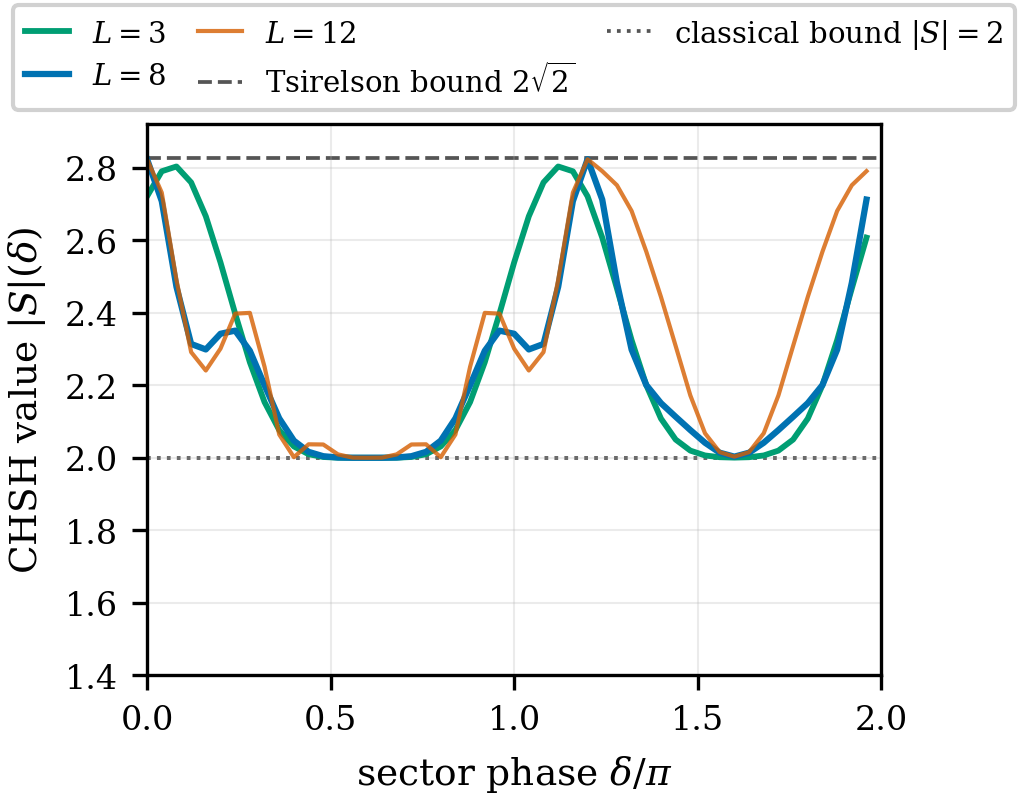
\includegraphics[width=\columnwidth]{figures/fig2_sector_phase.png}
\caption{\label{fig:sdelta}%
Sector-phase dependence $|S|(\delta)$ of the three-generator
sequences at braid lengths $L=3,8,12$ that maximize $|S|$ at $\delta = 0$
under Protocol~A (first maximizer in lexicographic order, from the
enumeration of all $3^L$ words). The CHSH value ranges from the
classical bound $|S|=2$ in the ``dead'' sector phases up to
$|S| = 2.824$ ($99.84\%$ of the Tsirelson bound $2\sqrt{2}$, dashed) at
$L = 8$ and $12$, where both curves reach this maximum at $\delta = 0$
and $\delta = 6\pi/5$ and lie on top of each other there; at $L = 3$ the
maximum is $2.804$. The curves at $L = 8$ and $12$ carry more structure
than at $L = 3$ (Fourier fits with four harmonics: $R^2 = 0.997$,
$0.837$, $0.914$; App.~\ref{app:fourier}). Lines connect the $N=50$
computed sector-phase points, so structure finer than the sampling is
not resolved. Data:
\texttt{s\_delta\_sweeps.json} (concept-DOI
10.5281/zenodo.19601352).}
\end{figure}

\begin{figure*}[!t]
\centering
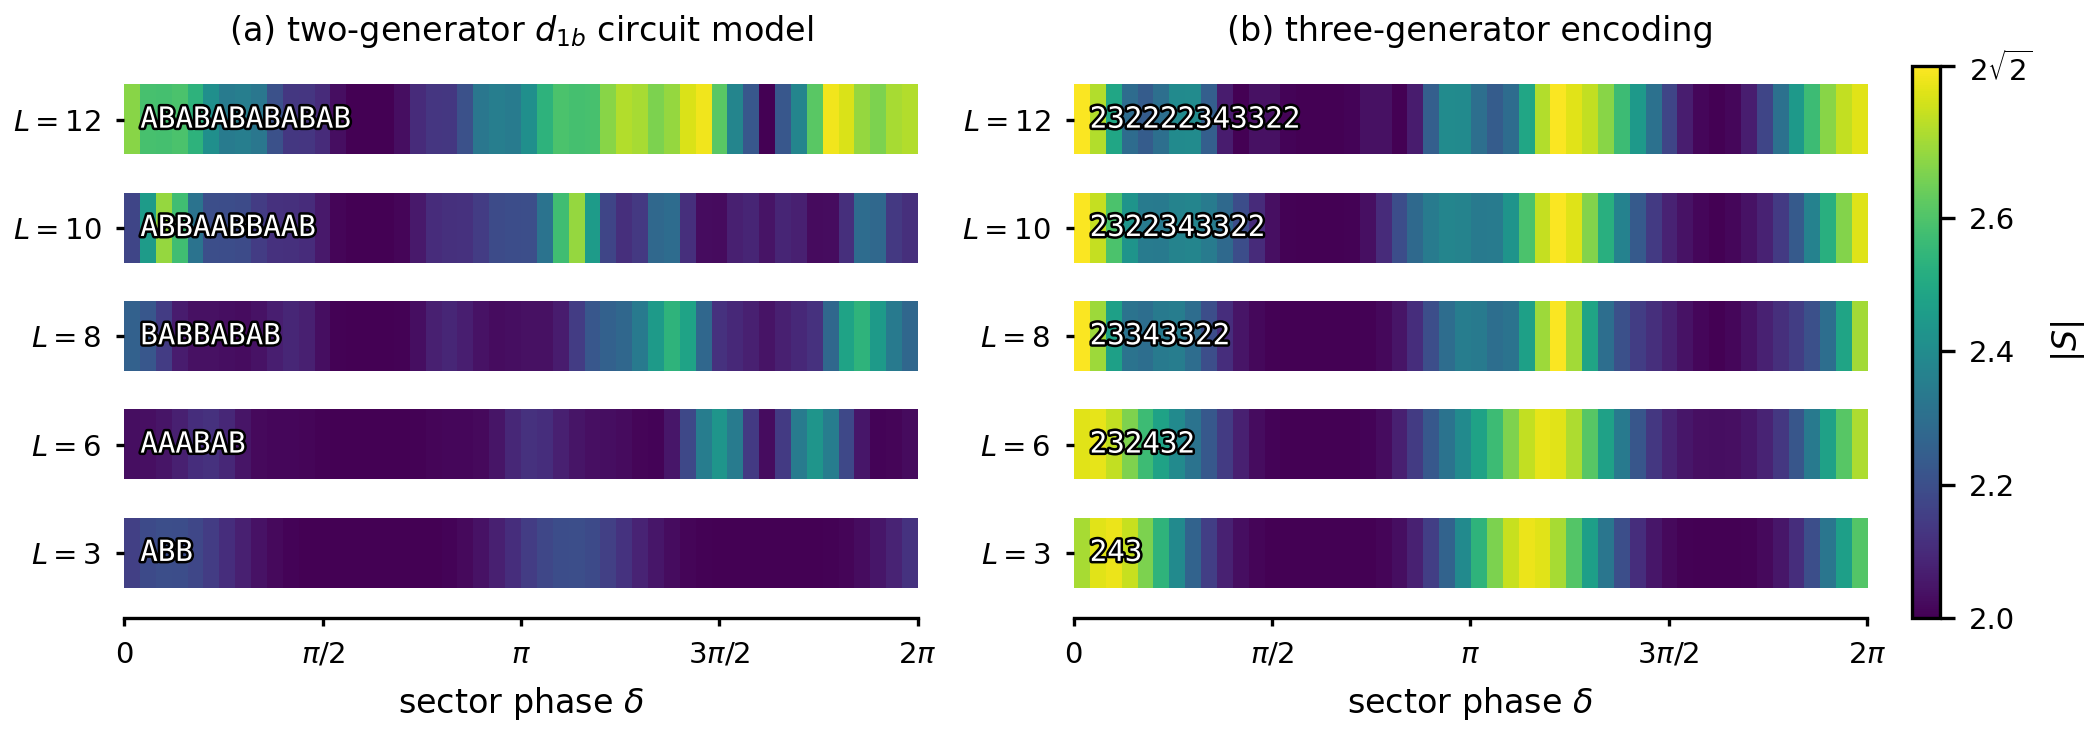
\includegraphics[width=\textwidth]{figures/fig4_sector_map.png}
\caption{\label{fig:sector_map}%
CHSH value $|S|$ of the sequence listed for each length (Table~\ref{tab:d1b}
for (a); for (b) the first $\delta = 0$ maximizer under Protocol~A) as a
function of the
sector phase $\delta$, for the two-generator $d_{1b}$ circuit model (a) and the
three-generator five-dimensional encoding (b). Each strip is one braid length;
$L$ is a categorical axis, since the deposited sweeps cover
$L \in \{3,6,8,10,12\}$ and nothing is drawn between them. Both panels share
one color scale, from the classical bound $|S| = 2$ to the Tsirelson bound
$2\sqrt{2}$.
Data: \texttt{s\_delta\_sweeps.json} (concept-DOI
10.5281/zenodo.19601352).}
\end{figure*}

At $L=2$, no sequence produces entanglement in the assignment
$\ket{11}\leftarrow\ket{4}$ ($C=0$): words without $\sigma_3$ consist of
gates local to Alice or Bob, and in words with $\sigma_3$ the generator
acts on a state supported on basis states that differ in one qubit only,
where it acts as a phase. The Protocol~A value $2.029$ of the word
$\sigma_2\sigma_4$ (Table~\ref{tab:3gen}) comes from the projection
alone.
From $L=3$ onward, the Protocol~A concurrence exceeds $0.92$ (rising to $0.997$
at $L=8$), reflecting the availability of $\sigma_3$ as a primitive
entangling gate.

The CHSH-violation fraction under 4D projection rises monotonically:
$44\%$ at $L=3$, $79\%$ at $L=6$, $92\%$ at $L=9$
(see Sec.~\ref{sec:protocol} for the protocol dependence of these
fractions).

\subsection{Comparing the two encodings}

The two encodings differ in the reachable group:
the circuit gates $\{\mathrm{AM},\mathrm{MB}\}$ generate a
six-dimensional proper subgroup of
$\mathrm{SU}(4)$ (entangling but not universal), whereas
$\{\sigma_2,\sigma_3,\sigma_4\}$ acts on the five-dimensional fusion space as
the standard $B_4$ braid representation, which is dense in
$\mathrm{SU}(2)\times\mathrm{SU}(3)$ on the two sectors of the intermediate
charge $x_2$~\cite{Bonesteel2005}; the four-dimensional computational-subspace
measurement is a projection of this action, not an invariant subspace. They
differ further in the word length required to approximate a given unitary.

In the three-generator encoding, $\sigma_3$ acts across the Alice--Bob
bipartition and provides the entangling step of the standard
\emph{rotate--entangle--rotate} decomposition. In the $d_{1b}$ circuit
model, the entangling step is the conditional gate MB, which is not a
braid; braiding with $\sigma_2$ and $\sigma_4$ alone does not entangle
(Sec.~\ref{sec:encodings}). The representation-dependence of the CHSH
operator norm on higher-dimensional Hilbert spaces is discussed in
Ref.~\cite{Sorella2023}.

%% ====================================================================
%% SECTION 4 — THE CROSS-BIPARTITION GENERATOR
%% ====================================================================
\section{The cross-bipartition generator $\sigma_3$}
\label{sec:switch}

We now show that, in the three-generator encoding, entanglement between
the logical qubits requires the generator $\sigma_3$.

\subsection{Blocking the cross-bipartition generator}

In the three-generator encoding, we replace $\sigma_3$\footnote{Index convention across the companion series: with $n=6$ anyons and the bipartition cut after anyon 3, the cross-bipartition generator of this paper is $\sigma_3$, while $\sigma_4$ acts locally on Bob's side. In the companion paper~\cite{Sayim2026chsh} ($n=8$ anyons, cut after anyon 4) the cross-bipartition role is played by its $\sigma_4$; the index shift is purely notational.} by the
$5\times 5$ identity matrix and evaluate the concurrence, with
$\ket{11}$ assigned to $\ket{4}$, on three representative
$\{\sigma_2,\sigma_4\}$ configurations, each swept over 50~linearly
spaced sector-phase values $\delta\in[0,2\pi)$
($150$ evaluations in total).

The result is absolute:
\begin{equation}
\label{eq:switch}
C(\mathcal{B},\delta)\big|_{\sigma_3\to I} = 0
\quad \forall\;\mathcal{B},\;\forall\;\delta.
\end{equation}
Across all tested blocked configurations (three representative
sequences at $L=3,6,8$ plus the $d_{1b}$ winner at $L=12$ with each
of its two generators blocked in turn, each configuration swept over
$50$ sector phases, totaling $5\times 50 = 250$
evaluations), the maximal concurrence is $C < 4.4\times 10^{-16}$
---machine zero.
Figure~\ref{fig:sigma3} contrasts the two cases for a representative
$L=8$ sequence $\sigma_2\sigma_3\sigma_4^4\sigma_3\sigma_2$: with
$\sigma_3$ active (Protocol~A), $|S|(\delta)$ rises above the classical
bound, up to $|S| = 2.808$ at $\delta/\pi = 1.24$ and $1.96$; with
$\sigma_3$ blocked, it is pinned to the classical bound for
every~$\delta$ in the assignment $\ket{11}\leftarrow\ket{4}$, and
reaches at most $|S| = 2.024$ under the Protocol~A projection, through
the projection alone.

\begin{figure}[t]
\centering
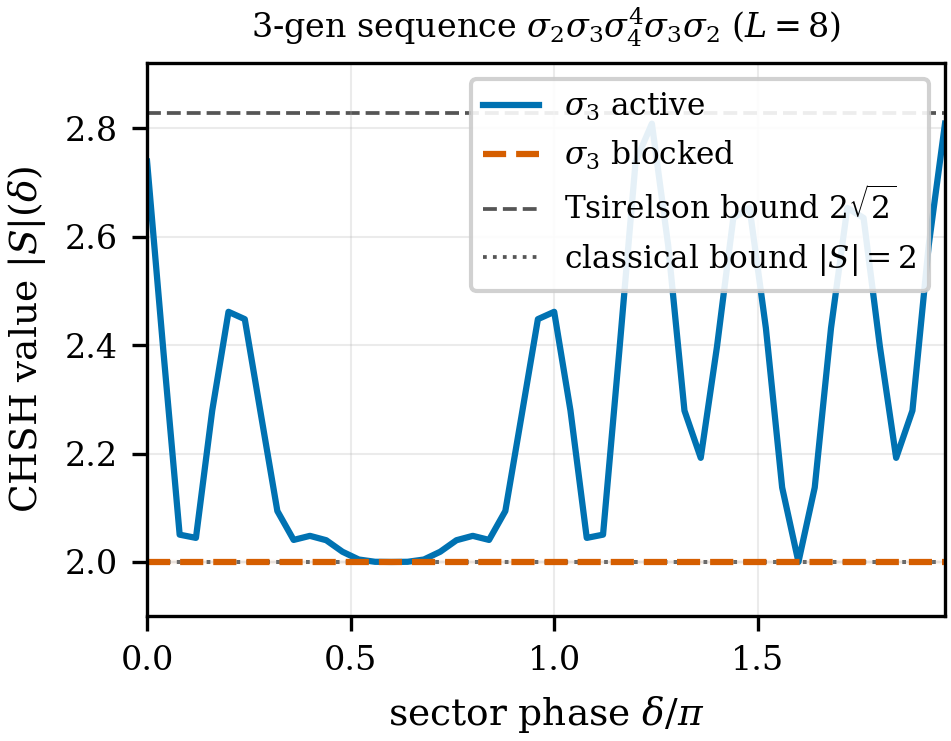
\includegraphics[width=\columnwidth]{figures/fig3_sigma3_switch.png}
\caption{\label{fig:sigma3}%
The $\sigma_3$ generator as a switch for entanglement, for a representative
$L=8$ three-generator sequence $\sigma_2\sigma_3\sigma_4^4\sigma_3\sigma_2$.
With $\sigma_3$ active (solid, Protocol~A), $|S|(\delta)$ rises above
the classical bound, up to $|S| = 2.808$ at $\delta/\pi = 1.24$ and
$1.96$; replacing $\sigma_3$ by the identity (dashed, assignment
$\ket{11}\leftarrow\ket{4}$) makes the concurrence vanish identically
[Eq.~\eqref{eq:switch}], pinning $|S|$ to the classical bound $|S|=2$
for every~$\delta$. Under the Protocol~A projection the blocked sequence
reaches at most $|S| = 2.024$, through the projection alone. Data: \texttt{topology\_switch\_results.json}
(concept-DOI 10.5281/zenodo.19601352).}
\end{figure}

\subsection{Physical mechanism}

The vanishing of entanglement under $\sigma_3$-blocking has a
transparent algebraic origin:
$\sigma_2$ preserves the $x_3$ label (Bob's qubit) and $\sigma_4$
preserves the $x_1$ label (Alice's qubit).
Without $\sigma_3$, which re-fuses the intermediate charge $x_2$ and
thereby couples the two branches of the fusion tree, the generators
act independently on the two logical qubits.
The resulting state is necessarily a product state, regardless of
sequence length or sector phase. This holds in the assignment
$\ket{11}\leftarrow\ket{4}$, in which $\sigma_2$ and $\sigma_4$ act as
single-qubit gates; the four-dimensional projection of Protocol~A
(Sec.~\ref{sec:protocol}) instead assigns
$\ket{11}\leftarrow(\ket{2}+\ket{4})/\sqrt{2}$, keeps only half of the
weight of $\ket{4}$, and can therefore report $C > 0$ for such product
states.

\subsection{The two-generator circuit model}

In the $d_{1b}$ circuit model, which has no $\sigma_3$, blocking either
$\text{AM}$ or $\text{MB}$ also collapses $C$ to zero exactly for the
optimal sequence $(\text{AM}\cdot\text{MB})^6$ at all 50~sector phases,
for a different reason: AM alone acts on Alice only, while MB alone
changes Bob's qubit conditioned on Alice's, which stays in $\ket{0}$
when AM is removed. Entanglement in the circuit model therefore requires
both gates.

\subsection{Interpretation}

In the three-generator encoding the $\sigma_3$ switch shows which
braiding operations make entanglement accessible: from the product input
state, only a generator acting across the bipartition can create it, as
in any quantum circuit acting on a product input.
Section~\ref{sec:sequential} returns to this result in a time-resolved
setting.



%% ====================================================================
%%  SECTION 5 — MEASUREMENT PROTOCOL AND LEAKAGE
%% ====================================================================
\section{Measurement protocol and computational-subspace leakage}
\label{sec:protocol}

The CHSH-violation fractions reported in Sec.~\ref{sec:reconciliation}
for the three-generator encoding depend on how observables are defined
in the five-dimensional fusion space.
We distinguish two measurement protocols and present results for both.

\subsection{Protocol~A: Computational-subspace projection}

The four-dimensional computational subspace is defined by identifying
the logical two-qubit basis as
$|00\rangle \leftarrow |0\rangle$,
$|01\rangle \leftarrow |1\rangle$,
$|10\rangle \leftarrow |3\rangle$, and
$|11\rangle \leftarrow (|2\rangle + |4\rangle)/\sqrt{2}$.
The last mapping coherently recombines the two basis states with
$x_1=\tau$, $x_3=\tau$ that differ only in the intermediate charge
$x_2$. Because a state without weight on $\ket{2}$ keeps only half of
its $\ket{4}$ weight under this mapping, the projection can turn a
product state into a non-product one: at $L=9$, $510$ of the $18\,064$
words that exceed $|S| = 2$ under Protocol~A contain no $\sigma_3$ and
exceed 2 only through the projection
(\texttt{d10\_protocol\_a\_projection\_audit.py}).
After projection and renormalization, the standard two-qubit
Horodecki criterion~\eqref{eq:horodecki} applies.

Under Protocol~A, the CHSH-violation fraction rises monotonically
with braid length and reaches $91.8\%$ at $L=9$
(Table~\ref{tab:protocol}).
The maximal CHSH value under Protocol~A saturates at $|S|=2.824$
(Table~\ref{tab:3gen}), within $0.16\%$ of the Tsirelson bound
$|S|=2\sqrt{2}$---approached but, per the exhaustive $3^8$-sequence
search, not exactly attained by any single braid word at $L=8$,
reflecting the residual cost of the four-dimensional
computational-subspace projection rather than a different physical
limit.

\subsection{Protocol~B: Native 5D CHSH}

We define Alice and Bob observables directly in the five-dimensional
fusion space:
\begin{align}
Z_A &= \text{diag}(+1,+1,-1,-1,-1), \label{eq:ZA} \\
Z_B &= \text{diag}(+1,-1,-1,+1,-1), \label{eq:ZB}
\end{align}
assigning eigenvalues $\pm 1$ according to the $x_1$ and $x_3$ labels.
The $X$-observables implement spin flips within each qubit sector:
$X_A$ swaps $|0\rangle\leftrightarrow|3\rangle$ and
$|1\rangle\leftrightarrow|4\rangle$, while $X_B$ swaps
$|0\rangle\leftrightarrow|1\rangle$ and
$|3\rangle\leftrightarrow|4\rangle$.
The state $|2\rangle = (\tau,1,\tau)$ has no flip partner in either
qubit sector, giving $X|2\rangle = 0$---i.e., the $X$ and $Y$
observables have spectrum $\{-1,0,+1\}$ (trit-valued).

We apply the Horodecki formula to the $3\times 3$ correlation matrix
$T_{ij} = \text{Re}\,\langle\psi|A_i \otimes B_j|\psi\rangle$,
yielding $|S|_{\max} = 2\sqrt{m_1+m_2}$ where $m_1,m_2$ are the
two largest eigenvalues of $T^T T$. Because the formula assumes
$\pm1$-valued observables on a two-qubit tensor product, which these
trit-valued observables on a single five-dimensional space are not, we
report the result as a Horodecki-type score rather than as a Bell test.
All observables commute across the bipartition ($[A_i,B_j]=0$ for all
$i,j$).

\subsection{Protocol comparison}

Table~\ref{tab:protocol} compares the two protocols across braid
lengths $L=3$--$9$ (exhaustive enumeration of all $3^L$ sequences).

\begin{table*}[!htb]
\caption{%
CHSH-violation statistics under two measurement protocols.
$|S|_{\max}$ is the largest CHSH value across all sequences.
CHSH\% counts sequences with $|S| > 2 + \tau$, $\tau = 10^{-10}$;
the ``at bound'' column counts those with $\bigl||S| - 2\bigr| \leq \tau$,
which are never assigned to either side.
$N^2_{\min}$ is the minimum computational-subspace fidelity.
Columns may not sum to $100$ due to rounding.
}
\label{tab:protocol}
\begin{ruledtabular}
\begin{tabular}{rccccccr}
$L$ & $|S|^{5\text{D}}_{\max}$ & $|S|^{4\text{D}}_{\max}$
& CHSH\%$_{5\text{D}}$ & at bound$_{5\text{D}}$
& CHSH\%$_{4\text{D}}$ & $\Delta$
& $N^2_{\min}$ \\
\hline
3 & 2.305 & 2.722 & 7.4 & 92.6 & 44.4 & +37.0 & 0.736 \\
4 & 2.305 & 2.722 & 9.9 & 80.2 & 61.7 & +51.9 & 0.635 \\
5 & 2.517 & 2.791 & 16.5 & 66.3 & 72.4 & +56.0 & 0.480 \\
6 & 2.517 & 2.791 & 23.6 & 53.4 & 79.0 & +55.4 & 0.281 \\
7 & 2.517 & 2.791 & 33.7 & 43.5 & 84.2 & +50.5 & 0.281 \\
8 & 2.517 & 2.824 & 39.1 & 35.6 & 88.5 & +49.4 & 0.183 \\
9 & 2.517 & 2.824 & 42.8 & 28.5 & 91.8 & +49.0 & 0.131 \\
\end{tabular}
\end{ruledtabular}
\end{table*}

\begin{figure*}[t]
\centering
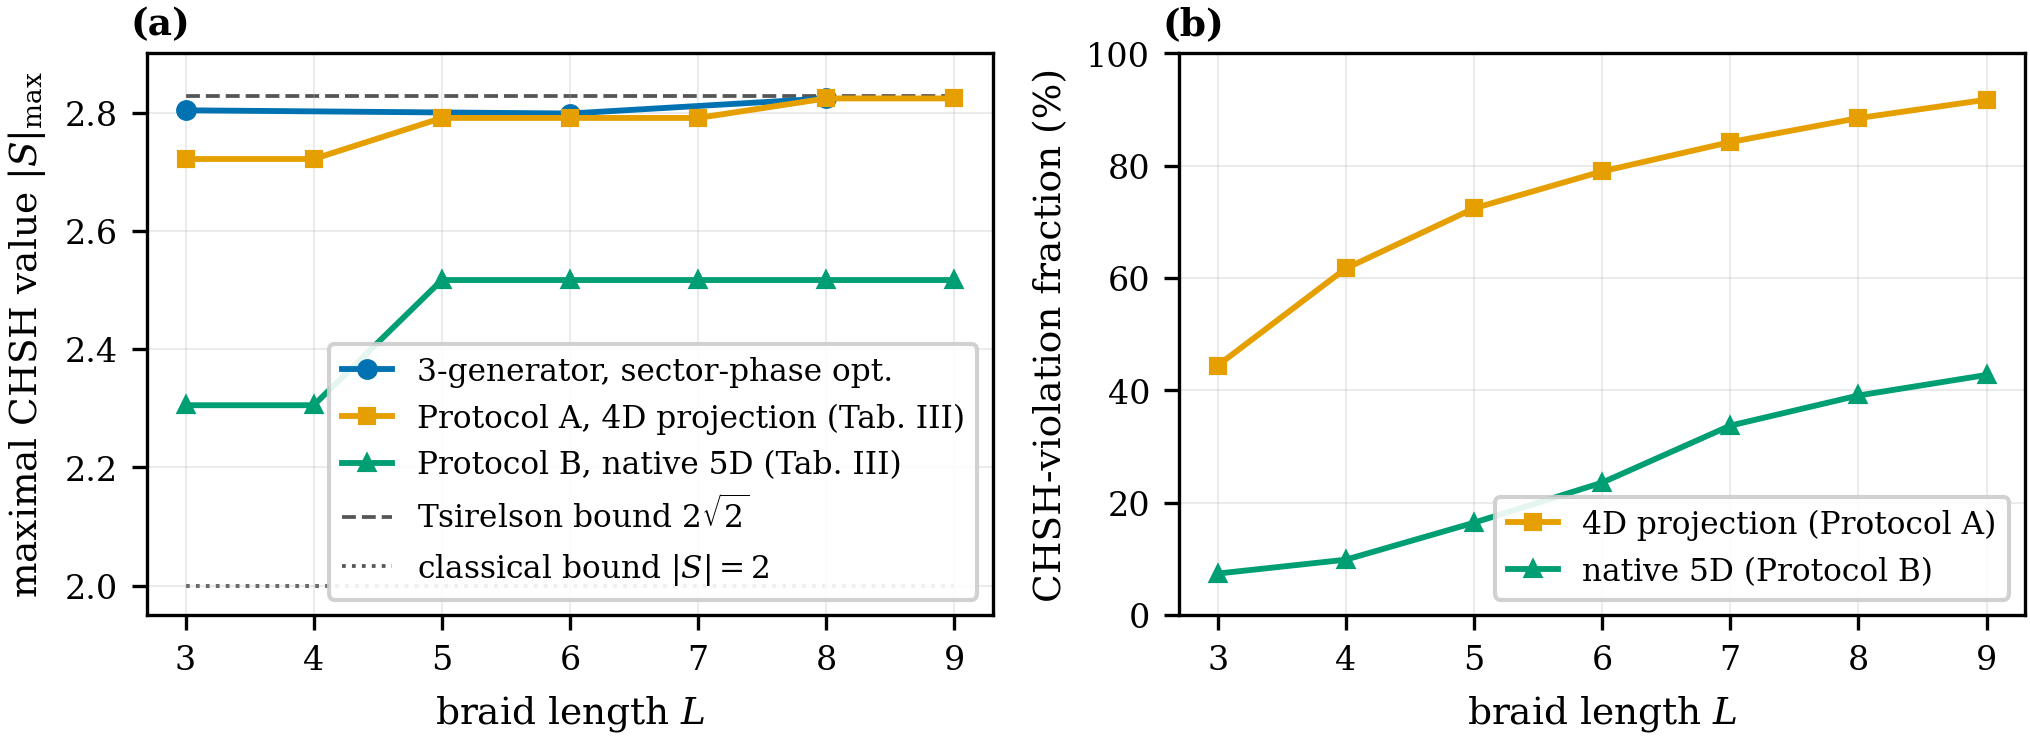
\includegraphics[width=0.9\textwidth]{figures/fig1_landscape.png}
\caption{\label{fig:landscape}%
Braiding-length dependence of the CHSH landscape.
(a)~Maximal CHSH value $|S|_{\max}$ versus braid length $L$ for the
three-generator encoding at the sector-phase optimum of the first
$\delta = 0$ maximizers under Protocol~A for $L = 3, 6, 8$ (per-$L$ maxima
of \texttt{s\_delta\_sweeps.json}: $2.804$, $2.798$, $2.824$; at $L = 8$
this point coincides with the Protocol~A value and lies beneath its
marker), and for
the two operational measurement protocols (Table~\ref{tab:protocol}):
Protocol~A (four-dimensional computational-subspace projection,
approaching $2\sqrt{2}$ within $0.16\%$) and Protocol~B (native
five-dimensional, trit-valued observables, saturating near $2.517$).
Dashed: Tsirelson bound $2\sqrt{2}$; dotted: classical bound $|S|=2$.
(b)~Fraction of braiding sequences with $|S| > 2 + \tau$ under the two
protocols. Both rise monotonically with $L$, reaching $91.8\%$
(Protocol~A) and $42.8\%$ (Protocol~B) at $L=9$; under Protocol~B a
further $28.5\%$ of sequences lie exactly at the classical bound. Data: \texttt{landscape\_validation.json}
and \texttt{s\_delta\_sweeps.json}
(concept-DOI
10.5281/zenodo.19601352).}
\end{figure*}

Figure~\ref{fig:landscape} summarizes both protocols across braid
length. The two protocols agree in direction---under both, the violating
fraction rises monotonically with $L$---but not in magnitude:
Protocol~A exceeds one half from $L=4$ onward, whereas Protocol~B
reaches $42.8\%$ at $L=9$. They differ in two further respects:

(i)~The maximal CHSH value in Protocol~B saturates at
$|S|^{5\text{D}}_{\max}\approx 2.517$ from $L=5$ onward,
while Protocol~A approaches the Tsirelson bound (within $0.16\%$).
The gap reflects the zero eigenvalue of the $X$ and $Y$ observables
on $|2\rangle$: a maximally entangled singlet-like state cannot be
fully realized in the five-dimensional space using trit-valued
observables.

(ii)~The CHSH fraction in Protocol~B rises monotonically to $42.8\%$ at
$L=9$, remaining below one half at every length, while under Protocol~A
it exceeds one half from $L=4$ onward.

\subsection{Leakage statistics}

The computational-subspace fidelity is the squared overlap onto the
orthonormal logical basis
$\{\ket{0},\ket{1},\ket{3},(\ket{2}+\ket{4})/\sqrt{2}\}$,
\begin{equation}
N^2 = |\psi_0|^2 + |\psi_1|^2 + |\psi_3|^2 + \tfrac{1}{2}|\psi_2+\psi_4|^2,
\end{equation}
which measures the fraction of the five-dimensional state that
survives projection into the two-qubit subspace and satisfies
$N^2\in[0,1]$ by construction.
At $L=9$, the minimum fidelity across all $19\,683$ sequences is
$N^2_{\min} = 0.131$, meaning that for some sequences up to $86.9\%$
of the amplitude resides outside the computational subspace.

This is consistent with the expectation that exact leakage-free
entangling gates may not exist for Fibonacci anyons~\cite{Cui2019}.
Protocol~A implicitly post-selects on the computational subspace by
renormalization; Protocol~B avoids this at the cost of a reduced
maximal $|S|$.

\subsection{Summary statement}

CHSH-form values above 2 are not confined to special braiding sequences
under either evaluation. Their frequency and size, however, depend on
the evaluation:
the CHSH fraction ($42.8\%$ vs.\ $91.8\%$ at $L=9$)
and the saturation value of $|S|_{\max}$ ($2.517$ vs.\ $2.824$)
both differ, reflecting the incomplete flip symmetry of the
five-dimensional fusion space and, for Protocol~A, the contribution of
the projection itself.

\textit{Note on terminology.}\, In this paper, ``Protocol~B'' refers
specifically to the bipartite native-$5$D CHSH evaluation with
trit-valued $Z$ and $X$-like observables on the full five-dimensional
fusion space (Sec.~\ref{sec:protocol}, this paper). Other companion
analyses that probe alternative nonbipartite CHSH constructions on
the same fusion space (e.g., minimal three-diagonal-parity
single-particle constructions) are distinct in scope and are not
covered by the present landscape; the bipartite Protocol~B used here
remains well-defined as a Horodecki-type score in its own right.

We emphasize that the $d_{1b}$ circuit model
(Sec.~\ref{sec:reconciliation}, Table~\ref{tab:d1b}) acts on a
four-dimensional space with no leakage and yields the sector-phase grid
maximum $|S|=2.811$ of the $d_{1b}$ circuit model ($\delta/\pi = 1.44$
and $1.76$); at $\delta = 0$, with the standard Fibonacci data, the $L =
12$ maximum is $|S| = 2.733$, the value adopted as the Fibonacci
reference in Ref.~\cite{Sayim2026topological}.

%% ====================================================================
%%  SECTION 6 — SEQUENTIAL BRAIDING
%% ====================================================================
\section{Sequential braiding and temporal correlations}
\label{sec:sequential}

We now show that sequential braiding on a shared fusion space produces
temporal correlations in the simulated CHSH-value series.

\subsection{Setup}

A register of six Fibonacci anyons is initialized in the vacuum state
$|0\rangle$ and subjected to $N=1000$ sequential braiding steps.
At each step~$n$, a generator $h_n\in\{\sigma_2,\sigma_3,\sigma_4\}$ is
drawn from a specified distribution, the state is updated as
$|\psi_n\rangle = h_n|\psi_{n-1}\rangle$, and its CHSH value under the
four-dimensional projection (Protocol~A, Sec.~\ref{sec:protocol}), $S_n =
S[\psi_n]$, is recorded.
This is repeated for $M=20$ independent runs.

Three models are compared:

\emph{Model~A} (i.i.d.):
each generator is chosen uniformly at random ($p=1/3$ each).

\emph{Model~B} (Markov-persistent):
with probability $0.6$, the previous generator is repeated;
otherwise a uniform draw from the remaining two.

\emph{Model~C} (no $\sigma_3$):
generators drawn from $\{\sigma_2,\sigma_4\}$ only ($p=1/2$ each),
serving as a control.

\subsection{Pillar~2: Null test}

As a prerequisite, we verify that \emph{independent} sector phases
produce no autocorrelation.
Drawing $N=10\,000$ sector phases $\delta_i$
uniformly from $[0,2\pi)$ and computing the CHSH value for each,
the lag-1 autocorrelation is
$\text{ACF}(1) = +0.002$ (Model~A configuration) and
$\text{ACF}(1) = +0.010$ (d1b configuration),
both within the $95\%$ confidence interval
$\pm 1.96/\sqrt{N} = \pm 0.020$
(seeded evaluation deposited as
\texttt{d8\_acf\_null\_robustness.py}).

The null hypothesis (ACF~$=0$ under i.i.d.\ sectors) is not
rejected.
This confirms that any nonzero autocorrelation observed in the
sequential-braiding models is a genuine dynamical effect, not
a statistical artifact.

\subsection{Pillar~3: Sequential-braiding autocorrelation}

Table~\ref{tab:acf} presents the measured autocorrelation for the
three models.

\begin{table}[!htb]
\caption{%
Lag-1 autocorrelation of the CHSH time series under sequential
braiding.
Significance is measured against the shuffle confidence band
(1000 random permutations of the observed series). CHSH values under
Protocol~A; CHSH\% is the fraction of steps with $|S| > 2 + 10^{-10}$. }
\label{tab:acf}
\begin{ruledtabular}
\begin{tabular}{lcccc}
Model & Generators & ACF(1) & Significance & CHSH\% \\
\hline
A (i.i.d.) & $\sigma_2,\sigma_3,\sigma_4$ & $+0.346$ & $11.22\sigma$ & 99.5 \\
B (Markov) & $\sigma_2,\sigma_3,\sigma_4$ & $+0.352$ & $10.53\sigma$ & 99.0 \\
C (no $\sigma_3$) & $\sigma_2,\sigma_4$ & $+0.035$ & $1.13\sigma$ & 81.0 \\
\end{tabular}
\end{ruledtabular}
\end{table}

Both Models~A and~B exhibit highly significant positive autocorrelation,
with Model~B only marginally above Model~A ($0.352$ vs.\ $0.346$).
This indicates that the autocorrelation arises primarily from
\emph{state continuity}---each braid step applies a finite rotation,
keeping $|\psi_n\rangle$ close to $|\psi_{n-1}\rangle$ in Hilbert
space---rather than from generator-level persistence.

Model~C shows no significant autocorrelation ($\text{ACF}(1)=+0.035$,
$1.13\sigma$). Its values are not constant under the four-dimensional
projection: the product states reached by $\sigma_2$ and $\sigma_4$ acquire a
nonzero projected concurrence, the same projection effect as for the $510$
words without $\sigma_3$ (Sec.~\ref{sec:protocol}), so $81\%$ of its values
lie above 2. In the natural assignment ($\ket{11}$ assigned to $\ket{4}$) the
concurrence stays zero and $|S|=2$ exactly, as in Sec.~\ref{sec:switch}.


\subsection{Robustness}

Replacing the vacuum initial state with a seeded random normalized
five-dimensional vector yields $\text{ACF}(1)=+0.314$ (Model~A) and $+0.336$
(Model~B), confirming that the effect survives
initialization.

The full autocorrelation range across the four deposited setups
(vacuum and random initialization, Models A and B) is
$\text{ACF}(1)\in [0.31,\,0.36]$, with the representative value for long runs
(Model~A, vacuum start) being $+0.35$.

\subsection{Summary of the three results}

The three pillars combine as follows:

\emph{Pillar~1} (Sec.~\ref{sec:switch}): $\sigma_3$-blocking shows
that, in the three-generator encoding, a single generator switches
entanglement on and off, as expected: without it, all gates are local.

\emph{Pillar~2} (this section): the null test confirms that
i.i.d.\ sector phases produce no autocorrelation---the method has
no intrinsic bias.

\emph{Pillar~3} (this section): sequential braiding produces
$\text{ACF}(1)=+0.35$ at $>10\sigma$---state continuity along the braid
sequence produces genuine temporal correlations of the simulated CHSH
value.

\subsection{Proposed experimental test}

In an experiment with sequential anyon braiding, the detection
sequence of CHSH-violation outcomes may exhibit positive
autocorrelation. We define the signed per-run CHSH term
\begin{equation}
g_n = (-1)^{a_n b_n}\, x_n y_n \in \{-1,+1\},
\end{equation}
where $a_n,b_n\in\{0,1\}$ label the measurement settings and
$x_n,y_n\in\{-1,+1\}$ the outcomes of run $n$; $\text{ACF}(1)$ denotes
the lag-1 autocorrelation of the $g_n$ series.
For independently re-prepared trials, such as the spacelike-separated
trials of loophole-free Bell
tests~\cite{Hensen2015,Giustina2015,Shalm2015}, no systematic positive
ACF is expected. The simulated value ($\text{ACF}(1)\approx 0.35$)
refers to the CHSH value of the state along the braid sequence,
evaluated with state-dependent optimal settings and with no measurement
between steps. An experiment records single-run CHSH terms $g_n$ and
measures in every run; whether a positive autocorrelation survives
measurement back-action, single-shot sampling noise and fixed settings
is not computed here, so $\text{ACF}>0$ for $g_n$ is a hypothesis to be
tested on platforms that braid sequentially on a shared fusion register,
not a derived prediction.

As a null control, we computed $\text{ACF}(1)$ on the published
outcome sequence of the openly available loophole-free test of Hensen
\emph{et al.}~\cite{Hensen2015} (data DOI
10.4121/uuid:6e19e9b2-4a2d-40b5-8dd3-a660bf3c0a31, $N=245$ valid
trials), finding
$\text{ACF}(1)=-0.047$ ($-0.64\sigma$, $|\text{ACF}(1)|<0.125$ at
$2\sigma$)---consistent with zero, as expected: the sequential-braiding
mechanism proposed here is structurally absent from independently
re-prepared Bell trials, so this is a genuine null control rather
than a failed prediction. The earlier test of Giustina \emph{et
al.}~\cite{Giustina2015} is closed as a venue for this analysis, as
its outcome sequence is available only on request; the higher-statistics
Shalm--NIST test~\cite{Shalm2015}, although also openly available, was
not analyzed here.
The appropriate venue to test the sequential-braiding hypothesis is
a platform that physically implements braiding sequentially on a
shared register, such as the digital Fibonacci-anyon realization of
Xu \emph{et al.}~\cite{XuEtAl2024} or the digital non-Abelian
Ising-anyon braiding of Andersen \emph{et al.}~\cite{Google2023};
both are gate-based (digital) realizations rather than the analog
continuous-braiding transport assumed in the present model, a
distinction relevant to any quantitative comparison.
The memory loophole in sequential Bell-type
data is well
characterized~\cite{BarrettCollinsHardyKentPopescu2002}; related but
distinct analyses of the same loophole-free data sets include a
no-signaling test~\cite{AdenierKhrennikov2017} and a
Kolmogorov-complexity analysis of the outcome
sequences~\cite{KovalskyHniloAguero2018,KovalskyHniloAguero2018b},
neither of which computes the lag-1 ACF proposed here; improved
statistical methodology for Bell-experiment data is discussed in
Ref.~\cite{Gill2022}.

%% ====================================================================
%%  SECTION 7 — DISCUSSION
%% ====================================================================
\section{Discussion}
\label{sec:discussion}

\subsection{Braiding, circuit, and the crossing generator}

The central finding of this work is that braiding alone does not
entangle the logical qubits of the two-generator encoding: its
generators act on different anyons and commute, and all $8190$ braid
words of length $L=1$--$12$ give $|S|=2$ exactly on the fusion code.
Entanglement appears once a gate acts across the bipartition---the
conditional gate of the $d_{1b}$ circuit model, or the braid generator
$\sigma_3$ of the three-generator encoding. In the latter, values above
2 are not confined to special sequences: under computational-subspace
projection more than half of all sequences exceed 2 for $L\geq 4$ (a
count that includes words without $\sigma_3$, which exceed 2 only
through the projection), and under the native five-dimensional score the
fraction is smaller but rises monotonically with braid length, to
$42.8\%$ at $L=9$, with a further $28.5\%$ exactly at the classical
value.

\subsection{The cross-bipartition generator}

In the three-generator encoding, the $\sigma_3$-blocking result shows
which braiding operations make entanglement accessible: $\sigma_3$ is
the only generator acting across the Alice--Bob bipartition, and without
it the concurrence stays exactly zero, as it must for gates local to
either side acting on a product input (in the assignment
$\ket{11}\leftarrow\ket{4}$). The companion analysis of
Ref.~\cite{Sayim2026topological} reports an association between sector
labels and CHSH values in classical $\mathbb{Z}_2$ lattice gauge theory,
which it finds to be a finite-size effect of nontopological origin.

\subsection{Implications for topological quantum computation}

The $\sigma_3$-blocking mechanism has a direct interpretation in
the context of topological quantum computing:
any braiding protocol that inadvertently excludes the
cross-bipartition generator will produce zero entanglement,
regardless of circuit depth.
The leakage analysis (Sec.~\ref{sec:protocol}) shows that this
concern extends beyond gate selection to the measurement
protocol, as up to $86.9\%$ of state weight can reside outside
the computational subspace.
This reinforces the finding of Cui \emph{et al.}~\cite{Cui2019}
that exact leakage-free entangling gates for Fibonacci anyons
may not exist.

\subsection{Limitations}

Several limitations qualify our results:

(i)~All computations are \emph{numerical simulations} within the
idealized Fibonacci TQFT at zero temperature and zero decoherence.
Topological protection is expected to suppress braiding-phase
noise~\cite{Nayak2008}. For a closed-form two-parameter degradation
model of our own, $|S| = 2\lambda^2\sqrt{1+v^4 C^2}$ (charge-survival
probability $\lambda$, dephasing visibility $v$, ideal concurrence
$C$), pure dephasing ($v<1$, $\lambda=1$) bounds $|S|$ from below by
the classical value 2 (attained only in the fully-dephased limit
$v\to0$) and never drives it below---the violation \emph{vanishes}
rather than surviving degraded. Only charge-changing quasiparticle poisoning ($\lambda<1$)
can push $|S|$ below~2, at the Werner-state
threshold~\cite{Horodecki1995} $\lambda^\ast=2^{-1/4}=0.8409$ for an
ideal ($C=1$) Bell state and $\lambda^\ast=0.8416$ for the actually
braided state ($C=0.9968$)---a poisoning tolerance of order $16\%$
per qubit before the classical bound is restored; this follows
directly from the Horodecki and Werner criteria and is not a new
bound. A gap-scaling trade-off follows if the thermal quasiparticle
poisoning rate is exponentially suppressed by the gap (Arrhenius factor
$e^{-\Delta/k_BT}$), as expected in thermal equilibrium with a spectral
gap; for Majorana-based devices, Ref.~\cite{KarzigColePikulin2021}
analyzes the realistic sources, nonequilibrium above-gap quasiparticles
and equilibrium subgap states, and we adopt the simple form for
$\nu=12/5$ by analogy. The universal $\nu=12/5$ Fibonacci candidate,
with a measured activation gap of order tens of mK~\cite{Zhang2012},
would then be thermally more fragile than the $\nu=5/2$ Ising state,
whose gap is comparatively robust but which is not computationally
universal. A nonequilibrium quasiparticle floor can
exceed the equilibrium poisoning rate by orders of magnitude in
realistic samples and is decoupled from temperature, so the
limitation is not purely thermal and does not vanish as $T\to 0$.
Two further factors pull in opposite directions: at $\nu=12/5$,
Landau-level mixing favors the $k=3$ Read--Rezayi phase over a competing
re-entrant integer quantum Hall phase~\cite{Mong2017}, while fractional
quantum Hall states at nearby fillings, observed in the first excited
Landau level~\cite{Pan2008}, could add poisoning channels. We do not
quote a specific operation-time bound: non-Abelian braiding at
$\nu=12/5$ has not been experimentally demonstrated, so any
timescale estimate would be conditional on an identification---
$\nu=12/5$ as the Fibonacci-anyon $k=3$ Read--Rezayi
state---that is numerically supported but not experimentally
confirmed~\cite{Mong2017,Zhu2015,Pakrouski2016}. Measurement
imperfections beyond this poisoning model are not addressed here.

(ii)~The sector phase $\delta$ entering via $R_\tau\to R_\tau\cdot
e^{i\delta}$ is a deformation of the representation; for generic $\delta
\neq 0$ it does not give a braid-group representation
(App.~\ref{app:algebra}).

(iii)~The fraction of sequences above 2 depends on the evaluation
(Sec.~\ref{sec:protocol}): $91.8\%$ under the four-dimensional
projection, which can itself raise product states above 2, and $42.8\%$
for the native five-dimensional Horodecki-type score.

(iv)~The simulated autocorrelation (Sec.~\ref{sec:sequential}) is
quantitatively setup-dependent ($\text{ACF}(1)\in [0.31,0.36]$ across
the four deposited setups), though qualitatively robust
($\text{ACF}>0$); its transfer to single-shot experimental outcomes is
not computed.

(v)~In the five-dimensional encoding, a Fourier fit with four
harmonics describes $S(\delta)$ at $L=3$ almost completely
($R^2=0.997$) but leaves part of the structure at $L=8$ and $12$
unexplained ($R^2=0.837$ and $0.914$; App.~\ref{app:fourier}).

\subsection{Comparison with the independent fusion-sector construction of Xu, Ye, and You}
\label{sec:xuyeyou_comparison}

Independently, Xu, Ye, and You~\cite{Xu2025}
have studied CHSH correlations on triplets of the Fibonacci-anyon
state $|\tau,\tau;1\rangle$ using a graded three-dimensional
fusion-sector Hilbert space $\mathcal{H}_1 \oplus \mathcal{H}_\tau$
with measurement operators of the form $A_\alpha = \operatorname{diag}(1,
[[\cos\alpha,\sin\alpha],[\sin\alpha,-\cos\alpha]])$ (their Eq.~(23)).
Their construction reaches
$|S|_{\max} = (4\sqrt{2}\varphi + 2)/\varphi^3 \approx 2.633$
with superactivation as the underlying phenomenon: a single copy of
$|\tau,\tau;1\rangle$ admits a local hidden-variable model, while three
copies activate Bell nonlocality. Their setup is bipartite under the
graded tensor product, with $A_\alpha$ block-diagonal across
$\mathcal{H}_1$ and $\mathcal{H}_\tau$. Tsirelson's bound $2\sqrt{2}$
applies in their setting; the value $2.633$ is sub-Tsirelson due to
nonuniform Schmidt weights of the three-copy state
(weight $2/\varphi^2 \approx 0.764$ on $\mathcal{H}_\tau \otimes \mathcal{H}_\tau$).

The present paper's $d_{1b}$ four-dimensional encoding, by contrast,
operates on a single copy of an entangled two-qubit circuit state with
concurrence $C = 0.988$, reaching $|S| = 2.811$ at $\delta/\pi = 1.76$
(at $\delta = 0$ the maximum over all words, $|S| = 2.733$, belongs to a
different word); this is the encoding-level two-qubit Horodecki value
$2\sqrt{1+C^2}$ for this concurrence. The two constructions address
different questions (multi-copy activation versus single-copy
circuit-model violation) and produce different but compatible values:
both respect Tsirelson's bound, and the difference reflects distinct
Schmidt structures of the underlying states. The value $|S| = 3.406$ of
the companion paper~\cite{Sayim2026chsh} belongs to a nonbipartite
construction that violates setting-locality and is therefore not subject
to Tsirelson's bound.

\subsection{Outlook}

The present enumeration is bounded at $L=12$ by the $3^L$ scaling;
other anyon models (Ising, $\text{SU}(2)_k$ for $k>3$) and experimental
autocorrelation data are not addressed here.
Whether the Kitaev honeycomb model~\cite{Kitaev2006}, which offers a
lattice setting in which both classical and quantum limits are accessible,
can bridge the present work with the $\mathbb{Z}_2$ results of
Ref.~\cite{Sayim2026topological} remains an open question.
A further open question, suggested by the Schmidt-rank-3 structure of
the Xu, Ye, You construction~\cite{Xu2025}, is whether a single-copy
Schmidt-rank-3 state in the five-dimensional fusion space could be
prepared by a different braiding protocol, and which CHSH values such a
state would yield compared with the present results: $|S| = 2.733$ with
the standard Fibonacci data and $|S| = 2.811$ at the sector-phase
optimum $\delta/\pi = 1.76$ in the two-generator circuit model, and $|S|
= 2.824$ in the three-generator encoding under four-dimensional
projection at $L = 8$.

%% ====================================================================
%%  CONCLUSION
%% ====================================================================
\section{Conclusion}
\label{sec:conclusion}

We have presented a complete sequence-by-sequence enumeration of
CHSH-form values across all Fibonacci anyon braiding words of length
$L=3$--$12$ (two generators) and $L=2$--$9$ (three generators, with the
$\delta = 0$ maxima also at $L = 10$ and $12$) in two
complementary encodings, in the broader landscape of qualitative
Bell-test constructions on Fibonacci/Ising and Majorana
platforms~\cite{Brennen2009,ChangChuMa2017,Drummond2014,RomitoGefen2017,ClarkeSauDasSarma2016}
and the independently analyzed three-copy fusion-sector
construction of Xu, Ye, and You~\cite{Xu2025}; a companion
Leggett--Garg-inequality letter using the same Fibonacci $F$- and
$R$-matrices, with $K_3$ values reaching $99.998\%$ of the L\"uders bound
$3/2$, is reported in Ref.~\cite{Sayim2026LGI}.

Braiding alone does not entangle the logical qubits of the two-generator
encoding: on the fusion code all $8190$ braid words of length
$L=1$--$12$ give $|S| = 2$ exactly, while the two-qubit circuit built
from the same data exceeds 2. In the three-generator encoding, values
above 2 are common: $91.8\%$ of the sequences exceed 2 under
computational-subspace projection at $L=9$ (including $510$ words
without $\sigma_3$ that do so only through the projection), and $42.8\%$
under the native five-dimensional score, where a further $28.5\%$ lie
exactly at the classical value.

In the $d_{1b}$ circuit model the $L=12$ maximum is $|S|=2.733$
($96.6\%$ of the Tsirelson bound $2\sqrt{2}$, $C=0.932$) with the
standard Fibonacci data ($\delta = 0$) and $|S|=2.811$ ($99.4\%$,
$C=0.988$) at the sector-phase optimum, while the three-generator
encoding under four-dimensional projection reaches $|S|=2.824$
($99.84\%$) at $L=8$.

In the three-generator encoding, removing the cross-bipartition
generator $\sigma_3$ leaves only gates local to Alice or Bob and, from
the product input state, collapses entanglement to zero exactly (with
$\ket{11}$ assigned to $\ket{4}$), independent of sequence length and
sector phase; in the $d_{1b}$ circuit model, removing either of its two
gates likewise gives $C=0$.

Sequential braiding on a shared anyon register produces positive
lag-1 autocorrelation of the simulated CHSH value ($\text{ACF}(1)=+0.35$ at
$11.22\sigma$), a signature of state continuity: the state is carried
from step to step, and each step applies a single generator. Whether
single-run outcomes in an experiment, with a measurement in every run,
retain a positive autocorrelation is not computed here
(Sec.~\ref{sec:sequential}).

We emphasize that the CHSH values reported here, while in excess of the
classical bound, should not be interpreted as Bell violations in
the EPR sense (cf.\ Sec.~\ref{fn:nonsep}): the underlying Fibonacci
fusion space does not factorize as a tensor product of local Alice and
Bob subsystems, and the classical-bound excess is more precisely
characterized as a signature of nonseparability in fusion space.

These findings indicate that the available braiding operations determine
whether CHSH-form values above 2 are accessible on the fusion space.

%% ====================================================================
%%  DATA AND CODE AVAILABILITY
%% ====================================================================
\section*{Notation}
\noindent Symbols used in this paper.
\small
\begin{ruledtabular}
\begin{tabular}{l p{0.72\columnwidth}}
Symbol & Meaning \\
\hline
$L$ & braiding sequence length \\
$|S|$ & magnitude of the CHSH functional \\
$C$ & concurrence of the two-qubit state \\
$\mathrm{AM},\,\mathrm{MB}$ & the two gates of the $d_{1b}$ circuit model: AM acts on Alice's qubit, MB on Bob's qubit conditioned on Alice's; they are not the braid generators $\sigma_2$, $\sigma_4$ \\
$\sigma_2,\sigma_3,\sigma_4$ & braid generators of the three-generator encoding; $\sigma_2$ and $\sigma_4$ alone act on the fusion code of the two-generator encoding \\
$d_{1b}$ & the two-generator encoding of six Fibonacci anyons \\
$\delta$ & sector phase, a deformation parameter introduced through $R_\tau\to R_\tau\,e^{i\delta}$; only $\delta=0$ is the standard theory \\
$\varphi$ & golden ratio, $(1+\sqrt5)/2$ \\
\end{tabular}
\end{ruledtabular}

\section*{Data and Code Availability}

The deterministic scripts and JSON output files that validate the
results reported in this paper are archived on Zenodo under the
concept DOI
\href{https://doi.org/10.5281/zenodo.19601352}{10.5281/zenodo.19601352}
(which always resolves to the latest version). Paper, figures, and data are released
under the Creative Commons Attribution 4.0 International (CC~BY~4.0)
license; the deposited source code is released under the Apache License 2.0
(see \texttt{LICENSE} and \texttt{LICENSE-CODE}).
The archive includes the three-generator (5D) landscape validation
and its leakage-norm reanchor (\texttt{landscape\_validation.py},
\texttt{n2\_reanchor.py}); the Protocol~A projection audit, including
the first $\delta = 0$ maximizers of the three-generator encoding for
$L = 3, 6, 8, 10, 12$ over all $3^L$ words
(\texttt{d10\_protocol\_a\_projection\_audit.py}); a closed-form
sector-phase sweep validation covering all rows of
Table~\ref{tab:d1b} and the three-generator $\delta = 0$ maximizers at
$L = 3, 6, 8, 10, 12$
(\texttt{d4\_s\_delta\_sweep\_validation.py}, run after \texttt{d10},
reproducing \texttt{s\_delta\_sweeps.json} and the printed table
values); the $\sigma_3$-blocking validation, including the exact
$\sigma_3$-block $C=0$ check (\texttt{d5\_topology\_switch\_validation.py},
reproducing \texttt{topology\_switch\_results.json}); the braiding-only
computation on the leakage-free fusion code and the Yang--Baxter
residua and distant commutator of the generators used here
(\texttt{d9\_fusion\_code\_braiding\_only.py}); the Fourier fits of
Appendix~\ref{app:fourier} (\texttt{d11\_fourier\_fit\_sweeps.py}); the
sequential-braiding autocorrelation of Table~\ref{tab:acf}
(\texttt{d6\_acf\_prediction\_sequential\_braiding.py}); the seeded
Pillar-2 null test and initialization-robustness evaluation of
Sec.~\ref{sec:sequential} (\texttt{d8\_acf\_null\_robustness.py}); an
independent null-control reanalysis of the Hensen \emph{et al.}\
(2015) loophole-free Bell data, including the underlying public
dataset (\texttt{d7\_acf\_hensen2015\_null\_control.py}); and the
scripts that draw Figs.~\ref{fig:sdelta}, \ref{fig:sigma3}
and~\ref{fig:landscape} (\texttt{figures/make\_1b\_figs.py}) and
Fig.~\ref{fig:sector_map} (\texttt{figures/make\_1b\_fig4\_map.py}) from
the deposited JSON files. The two-generator sequences of
Table~\ref{tab:d1b} come from the full enumeration deposited with the
companion record~\cite{Sayim2026topological}. The checks of the
remaining generator pairs in Appendix~\ref{app:algebra} and the
$\mathbb{Z}_5$ phase spectrum of $\Delta^2$ were made with two further
scripts that are not part of this record.

%% ====================================================================
%%  USE OF AI TOOLS
%% ====================================================================
\section*{Use of AI tools}

In the research, processing, and writing of this paper and its results I worked together with generative AI tools, in practice a system of multiple coordinated AI instances that I set up and orchestrate (large language models, mainly Claude, by Anthropic, inside Claude Code). At their current context sizes I found it far more effective to work with several specialized instances, each with its own role and its own harness of rules and parameters that I designed and refined through feedback, than to load a single instance with all of the material; for my workflow that would have been inefficient, though this depends on the individual implementation. I lead this collaboration: I choose the research directions, set the goals, and make the final decisions in open exchange with the AI, learning actively as the work proceeds. The AI carries out the drafting, including the mathematical and technical parts, the numerical computation, and the literature search, under my direction. The AI works autonomously only task by task, within the structure I develop through feedback: it completes a task, and at open questions that need me it stops until the point is settled before the next step. Along the way I witness and take many of the decisions that shape the path, and it is common for me to spot things that need improvement. The work spans many separate runs, and a single simulation or build task alone can take up to an hour, so it could not happen all together in one autonomous run; and had I let the AI do all of it together alone, even if it is possible, it would no longer be my work but the AI's.

I run multiple verifications at the different stages of the work and one before release, including cross-checks with an unrelated AI model from a different company, and all references are checked against the original sources. In the end what matters are human eyes, a principle that is itself written into the parameters of my system: I reach out to experts after publishing for review and feedback, so I learn what is solid and what must be corrected or falsified. My scripts for reproduction and review are released with this record. These tools are not authors; I am the author, and I take full responsibility for all scientific content and decisions leading to these results and their publication.

%% ====================================================================
%%  ACKNOWLEDGMENTS
%% ====================================================================
\section*{Acknowledgments}
This research received no specific grant from any funding agency in the
public, commercial, or not-for-profit sectors. The author declares no
competing interests.

%% ====================================================================
%%  APPENDIX
%% ====================================================================
\appendix

\section{Braid-generator matrices}
\label{app:generators}

The five braid generators $\sigma_1,\ldots,\sigma_5$ for six
Fibonacci anyons in the basis~\eqref{eq:basis} are constructed
as follows.
For each generator $\sigma_k$, the anyon pair $(\tau_k,\tau_{k+1})$
is braided via the $F$-move/R-phase/$F$-move sequence on the
relevant two-dimensional subspace of the fusion tree.
The remaining basis states acquire diagonal $R$-phases.
Explicit $5\times 5$ matrices are provided in the supplementary
code archived with the Zenodo deposit.

The key structural properties:
\begin{itemize}
\item $\sigma_2$ mixes states within the $x_1\in\{1,\tau\}$
subspace (Alice's qubit), preserving $x_3$.
\item $\sigma_4$ mixes states within the $x_3\in\{1,\tau\}$
subspace (Bob's qubit), preserving $x_1$.
\item $\sigma_3$ re-fuses the intermediate label $x_2$, coupling
both branches of the fusion tree.
\item $\sigma_1$ and $\sigma_5$ act as diagonal phases on $x_1$
and $x_3$ respectively.
\end{itemize}

\section{Fourier structure of $S(\delta)$}
\label{app:fourier}

The CHSH value as a function of sector phase $\delta$ exhibits
encoding-dependent harmonic structure.
For the Ising anyon model, the functional form is exactly
$S(\delta) = 2\sqrt{2}\cos^2(\delta/2)$, containing only the
fundamental harmonic $n=1$. This idealized Ising result assumes
access to a nonstabilizer (``magic'') single-qubit operation beyond
the topologically protected Clifford gate set; purely stabilizer
operations on Ising anyons cannot violate the CHSH
inequality~\cite{HowardVala2012}.
For Fibonacci anyons we fit the deposited five-dimensional sweeps of
the first $\delta = 0$ maximizers at $L = 3$, $8$ and $12$
(Fig.~\ref{fig:sdelta}) by least squares with $N = 1,\dots,6$ harmonics,
\begin{equation}
S(\delta_k) \approx a_0 + \sum_{n=1}^{N}
\left(a_n\cos n\delta_k + b_n\sin n\delta_k\right),
\qquad \delta_k = 2\pi k/50,
\label{eq:fourier}
\end{equation}
(\texttt{d11\_fourier\_fit\_sweeps.py}; two solution routes agree to
$5\times10^{-16}$). With $N = 4$ the coefficient of determination is
$R^2 = 0.997$, $0.837$ and $0.914$ at $L = 3$, $8$ and $12$; with
$N = 6$ it is $1.000$, $0.919$ and $0.952$. For every $N \geq 2$ the
largest harmonic is $n = 2$, with amplitude
$\sqrt{a_2^2+b_2^2} = 0.388$, $0.280$ and $0.273$, and the constant term
is the mean of the curve ($a_0 = 2.280$, $2.243$, $2.315$). For
Fibonacci, generic $\delta \neq 0$ is a deformation that does not
preserve the braid relations (App.~\ref{app:algebra}), so we attach no
physical meaning to the harmonic content of these fits; they describe
the numerical curves only.

\section{Verification of the five-dimensional representation under sector-phase modulation}
\label{app:algebra}

The qualitative nonseparability and contextuality framing of Sec.~\ref{fn:nonsep} and
Sec.~\ref{sec:encodings} is supported by an independent numerical check
of the braid-group relations for the full five-state generators
$\sigma_1, \ldots, \sigma_5$ across a range of sector phases $\delta$.
At $\delta = 0$ the standard Fibonacci modular tensor category is
satisfied to floating-point precision (Yang--Baxter residuum below $10^{-15}$,
distant commutators identically zero).
Under the sector-phase modulation
$R_\tau \mapsto R_\tau \cdot e^{i\delta}$ introduced in
Sec.~\ref{sec:encodings}, Yang--Baxter deforms uniformly across
all four neighboring generator pairs while distant commutators
$[\sigma_i, \sigma_j] = 0$ for $|i-j| \geq 2$ remain identically zero
throughout. Table~\ref{tab:yb_under_delta} summarizes the verification.
The sector phase $\delta$ is thus a free deformation knob rather than a
physical parameter: generic $\delta \neq 0$ breaks the Yang--Baxter/hexagon
consistency of the representation (Table~\ref{tab:yb_under_delta}), and only
$\delta = 0$ recovers the standard Fibonacci modular tensor category. This
expected discreteness --- rather than a continuum of consistent deformations
--- is consistent with the general Ocneanu-rigidity result for fusion
categories~\cite{EtingofNikshychOstrik2002}, which here rests on the
paper-internal numerics of Table~\ref{tab:yb_under_delta} rather than on an
independent categorical classification of this specific representation.

On the 50-point grid the braid relations hold exactly only at
$\delta/\pi = 0$, $0.6$ and $1.2$: at $\delta = 3\pi/5$ all generators
become multiples of the identity, and at $\delta = 6\pi/5$ they are the
complex conjugates of the $\delta = 0$ generators up to a global phase.
Everywhere else on the grid the Yang--Baxter residuum is at least
$0.196$ (\texttt{d9\_fusion\_code\_braiding\_only.py}). More generally,
complex conjugation maps the braid generators at $\delta$ to those at
$6\pi/5 - \delta$ up to a global phase, and concurrence is invariant
under complex conjugation; numerically, every $|S|(\delta)$ sweep of
this paper, in both encodings, is mirror-symmetric about $\delta =
3\pi/5$ and $8\pi/5$ (deviation below $10^{-14}$), which is why the
$d_{1b}$ optimum appears twice, at $\delta/\pi = 1.44$ and $1.76$.

\begin{table}[h]
\caption{Algebraic verification of the five-state representation under
sector-phase modulation. The Yang--Baxter residuum
$\|\sigma_i\sigma_{i+1}\sigma_i - \sigma_{i+1}\sigma_i\sigma_{i+1}\|_F$
is identical across all four neighboring pairs and is shown in column 2.
The distant commutator $\|[\sigma_i, \sigma_j]\|_F$ for $|i-j| \geq 2$
vanishes for every tested $\delta$, as the block structure of the
generators requires; the deposited check of $[\sigma_2,\sigma_4]$, the
pair used in this paper, finds at most $8\times10^{-17}$, i.e.\
floating-point rounding.}
\label{tab:yb_under_delta}
\begin{ruledtabular}
\begin{tabular}{rcc}
$\delta/\pi$ & YB residuum (5D) & distant commutator (5D) \\
\hline
$0.000$ & $< 10^{-15}$ & $< 10^{-16}$ \\
$0.100$ & $0.525$ & $< 10^{-16}$ \\
$0.250$ & $0.958$ & $< 10^{-16}$ \\
$0.500$ & $0.474$ & $< 10^{-16}$ \\
$1.000$ & $0.873$ & $< 10^{-16}$ \\
$1.191$ & $0.052$ & $< 10^{-16}$ \\
$1.500$ & $1.523$ & $< 10^{-16}$ \\
\end{tabular}
\end{ruledtabular}
\end{table}

The intact $\delta = 0$ representation confirms that the noncommuting
$d_{1b}$ gates belong to the circuit model, not to the braid
representation (Sec.~\ref{sec:encodings}): in the fusion code,
$\sigma_2$ and $\sigma_4$ commute exactly.
The exact preservation of distant commutativity
under $\delta$-modulation is structural: the modulation acts locally
on the $R_\tau$ eigenvalue and does not couple block- or
diagonally-separated generators.
The Yang--Baxter residua of the generators used in this paper and
their distant commutator are recomputed by the deposited script
\texttt{d9\_fusion\_code\_braiding\_only.py}, which finds the commutator
below $10^{-16}$ at every tested $\delta$, as the structural argument
requires. The remaining pairs, the $\mathbb{Z}_5$ phase spectrum of
$\Delta^2$ from the Birman formula and the $d_{1b}$ spectator-filter
algebra-breaks were computed with two further scripts
(\texttt{d2\_delta\_phase\_consistency.py},
\texttt{d3\_5d\_braid\_algebra\_consistency.py}) that are not part of
this record.

%% ====================================================================
%%  REFERENCES
%% ====================================================================

\begin{thebibliography}{44}

\bibitem{Sayim2026topological}
B.~Y.~Sayim,
\emph{CHSH-form values above 2 for standard Fibonacci anyons, and the
non-topological origin of finite-size sector--CHSH mutual information in
$\mathbb{Z}_2$ lattice gauge theory},
Zenodo preprint (2026),
\href{https://doi.org/10.5281/zenodo.19600752}{doi:10.5281/zenodo.19600752}.

\bibitem{Sayim2026chsh}
B.~Y.~Sayim,
\emph{CHSH-form values without Bell nonlocality: Inapplicability of the
Tsirelson bound on a non-factorized Fibonacci fusion space},
Zenodo preprint (2026),
\href{https://doi.org/10.5281/zenodo.19601998}{doi:10.5281/zenodo.19601998}.

\bibitem{Nayak2008}
C.~Nayak, S.~H.~Simon, A.~Stern, M.~Freedman, and S.~Das~Sarma,
\emph{Non-Abelian anyons and topological quantum computation},
Rev.\ Mod.\ Phys.\ \textbf{80}, 1083 (2008).

\bibitem{Freedman2003}
M.~H.~Freedman, A.~Kitaev, M.~J.~Larsen, and Z.~Wang,
\emph{Topological quantum computation},
Bull.\ Am.\ Math.\ Soc.\ \textbf{40}, 31 (2003).

\bibitem{Bonesteel2005}
N.~E.~Bonesteel, L.~Hormozi, G.~Zikos, and S.~H.~Simon,
\emph{Braid topologies for quantum computation},
Phys.\ Rev.\ Lett.\ \textbf{95}, 140503 (2005).

\bibitem{Hormozi2007}
L.~Hormozi, G.~Zikos, N.~E.~Bonesteel, and S.~H.~Simon,
\emph{Topological quantum compiling},
Phys.\ Rev.\ B \textbf{75}, 165310 (2007).

\bibitem{Horodecki1995}
R.~Horodecki, P.~Horodecki, and M.~Horodecki,
\emph{Violating Bell inequality by mixed spin-$\frac{1}{2}$
states: necessary and sufficient condition},
Phys.\ Lett.\ A \textbf{200}, 340 (1995).

\bibitem{Cui2019}
S.~X.~Cui, K.~T.~Tian, J.~F.~Vasquez, Z.~Wang, and H.~M.~Wong,
\emph{The search for leakage-free entangling Fibonacci braiding gates},
J.\ Phys.\ A: Math.\ Theor.\ \textbf{52}, 455301 (2019);
\href{https://arxiv.org/abs/1904.01731}{arXiv:1904.01731}.

\bibitem{Burke2024}
P.~C.~Burke, C.~Aravanis, J.~Aspman, J.~Mare\v{c}ek, and J.~Vala,
\emph{Topological quantum compilation of two-qubit gates},
Phys.\ Rev.\ A \textbf{110}, 052616 (2024);
\href{https://arxiv.org/abs/2408.07132}{arXiv:2408.07132}.

\bibitem{Yang2019}
Z.-C.~Yang, K.~Meichanetzidis, S.~Kourtis, and C.~Chamon,
\emph{Scrambling via braiding of nonabelions},
Phys.\ Rev.\ B \textbf{99}, 045132 (2019).

\bibitem{Google2023}
T.~I.~Andersen \emph{et al.} (Google Quantum AI and Collaborators),
\emph{Non-Abelian braiding of graph vertices in a
superconducting processor},
Nature \textbf{618}, 264 (2023);
\href{https://arxiv.org/abs/2210.10255}{arXiv:2210.10255}.


\bibitem{Hensen2015}
B.~Hensen, H.~Bernien, A.~E.~Dr\'eau, A.~Reiserer, N.~Kalb, M.~S.~Blok,
J.~Ruitenberg, R.~F.~L.~Vermeulen, R.~N.~Schouten, C.~Abell\'an,
W.~Amaya, V.~Pruneri, M.~W.~Mitchell, M.~Markham, D.~J.~Twitchen,
D.~Elkouss, S.~Wehner, T.~H.~Taminiau, and R.~Hanson,
\emph{Loophole-free Bell inequality violation using electron
spins separated by 1.3 kilometres},
Nature \textbf{526}, 682 (2015).

\bibitem{Giustina2015}
M.~Giustina, M.~A.~M.~Versteegh, S.~Wengerowsky, J.~Handsteiner,
A.~Hochrainer, K.~Phelan, F.~Steinlechner, J.~Kofler,
J.-\AA{}.~Larsson, C.~Abell\'an, W.~Amaya, V.~Pruneri, M.~W.~Mitchell,
J.~Beyer, T.~Gerrits, A.~E.~Lita, L.~K.~Shalm, S.~W.~Nam, T.~Scheidl,
R.~Ursin, B.~Wittmann, and A.~Zeilinger,
\emph{Significant-loophole-free test of Bell's theorem with
entangled photons},
Phys.\ Rev.\ Lett.\ \textbf{115}, 250401 (2015).


\bibitem{Kitaev2006}
A.~Kitaev,
\emph{Anyons in an exactly solved model and beyond},
Ann.\ Phys.\ \textbf{321}, 2 (2006).



\bibitem{Brennen2009}
G.~K.~Brennen, S.~Iblisdir, J.~K.~Pachos, and J.~K.~Slingerland,
\emph{Non-locality of non-Abelian anyons},
New J.\ Phys.\ \textbf{11}, 103023 (2009);
\href{https://arxiv.org/abs/0810.4319}{arXiv:0810.4319}.

\bibitem{ChangChuMa2017}
P.-Y.~Chang, S.-K.~Chu, and C.-T.~Ma,
\emph{Bell's inequality and entanglement in qubits},
J.\ High Energy Phys.\ \textbf{09} (2017) 100;
\href{https://arxiv.org/abs/1705.06444}{arXiv:1705.06444}.

\bibitem{Drummond2014}
D.~E.~Drummond, A.~A.~Kovalev, C.-Y.~Hou, K.~Shtengel, and L.~P.~Pryadko,
\emph{Demonstrating entanglement by testing Bell's theorem in Majorana wires},
Phys.\ Rev.\ B \textbf{90}, 115404 (2014);
\href{https://arxiv.org/abs/1403.0916}{arXiv:1403.0916}.

\bibitem{RomitoGefen2017}
A.~Romito and Y.~Gefen,
\emph{Ubiquitous nonlocal entanglement with Majorana zero modes},
Phys.\ Rev.\ Lett.\ \textbf{119}, 157702 (2017);
\href{https://arxiv.org/abs/1703.01841}{arXiv:1703.01841}.

\bibitem{ClarkeSauDasSarma2016}
D.~J.~Clarke, J.~D.~Sau, and S.~Das~Sarma,
\emph{A practical phase gate for producing Bell violations in Majorana wires},
Phys.\ Rev.\ X \textbf{6}, 021005 (2016);
\href{https://arxiv.org/abs/1510.00007}{arXiv:1510.00007}.

\bibitem{Xu2025}
C.-Q.~Xu, W.~Ye, and L.~You,
\emph{Superactivation of Bell nonlocality in pure anyonic states},
Phys.\ Rev.\ A \textbf{112}, 062232 (2025);
\href{https://arxiv.org/abs/2506.08919}{arXiv:2506.08919}.

\bibitem{Sorella2023}
S.~P.~Sorella,
\emph{On the representations of Bell's operators in quantum mechanics},
Found.\ Phys.\ \textbf{53}, 59 (2023);
\href{https://arxiv.org/abs/2304.05696}{arXiv:2304.05696}.

\bibitem{Sayim2026LGI}
B.~Y.~Sayim,
\emph{Leggett--Garg $K_{3}$ values above 1 in Fibonacci-anyon braiding:
$99.998\%$ of the L\"uders bound, and exactly 1 for Ising braiding},
Zenodo preprint (2026),
\href{https://doi.org/10.5281/zenodo.20372744}{doi:10.5281/zenodo.20372744}.


\bibitem{GuimaraesRoditiSorella2024}
M.~S.~Guimaraes, I.~Roditi, and S.~P.~Sorella,
\emph{Bell-CHSH inequality and unitary operators},
Nucl.\ Phys.\ B (2024);
\href{https://arxiv.org/abs/2403.15276}{arXiv:2403.15276}.

\bibitem{Chou2025}
T.-M.~Chou,
\emph{Topological contextuality and quantum representations},
Int.\ J.\ Topol.\ \textbf{3}, 3 (2026);
\href{https://arxiv.org/abs/2506.14537}{arXiv:2506.14537}.

\bibitem{ShapourianMongRyu2020}
H.~Shapourian, R.~S.~K.~Mong, and S.~Ryu,
\emph{Anyonic partial transpose I: Quantum information aspects},
\href{https://arxiv.org/abs/2012.02222}{arXiv:2012.02222} (2020).

\bibitem{BondersonKnappPatel2017}
P.~Bonderson, C.~Knapp, and K.~Patel,
\emph{Anyonic entanglement and topological entanglement entropy},
Ann.\ Phys.\ \textbf{385}, 399 (2017);
\href{https://arxiv.org/abs/1706.09420}{arXiv:1706.09420}.

\bibitem{EtingofNikshychOstrik2002}
P.~Etingof, D.~Nikshych, and V.~Ostrik,
\emph{On fusion categories},
Ann.\ of Math.\ \textbf{162}, 581--642 (2005);
\href{https://arxiv.org/abs/math/0203060}{arXiv:math/0203060}.

\bibitem{KarzigColePikulin2021}
T.~Karzig, W.~S.~Cole, and D.~I.~Pikulin,
\emph{Quasiparticle poisoning of Majorana qubits},
Phys.\ Rev.\ Lett.\ \textbf{126}, 057702 (2021).

\bibitem{Mong2017}
R.~S.~K.~Mong, M.~P.~Zaletel, F.~Pollmann, and Z.~Papi\'{c},
\emph{Fibonacci anyons and charge density order in the 12/5 and 13/5 plateaus},
Phys.\ Rev.\ B \textbf{95}, 115136 (2017);
\href{https://arxiv.org/abs/1505.02843}{arXiv:1505.02843}.

\bibitem{Zhang2012}
C.~Zhang, C.~Huan, J.~S.~Xia, N.~S.~Sullivan, W.~Pan, K.~W.~Baldwin, K.~W.~West, L.~N.~Pfeiffer, and D.~C.~Tsui,
\emph{Spin polarization of the $\nu=12/5$ fractional quantum Hall state},
Phys.\ Rev.\ B \textbf{85}, 241302(R) (2012);
\href{https://arxiv.org/abs/1204.0560}{arXiv:1204.0560}.

\bibitem{Pakrouski2016}
K.~Pakrouski, M.~Troyer, Y.-L.~Wu, S.~Das~Sarma, and M.~R.~Peterson,
\emph{The enigmatic 12/5 fractional quantum Hall effect},
Phys.\ Rev.\ B \textbf{94}, 075108 (2016);
\href{https://arxiv.org/abs/1604.04610}{arXiv:1604.04610}.

\bibitem{Zhu2015}
W.~Zhu, S.~S.~Gong, F.~D.~M.~Haldane, and D.~N.~Sheng,
\emph{Fractional quantum Hall states at $\nu=13/5$ and $12/5$ and their
non-Abelian nature}, Phys.\ Rev.\ Lett.\ \textbf{115}, 126805 (2015);
\href{https://arxiv.org/abs/1505.03050}{arXiv:1505.03050}.

\bibitem{Pan2008}
W.~Pan, J.~S.~Xia, H.~L.~Stormer, D.~C.~Tsui, C.~Vicente, E.~D.~Adams, N.~S.~Sullivan, L.~N.~Pfeiffer, K.~W.~Baldwin, and K.~W.~West,
\emph{Experimental studies of the fractional quantum Hall effect in the first excited Landau level},
Phys.\ Rev.\ B \textbf{77}, 075307 (2008);
\href{https://arxiv.org/abs/0801.1318}{arXiv:0801.1318}.


\bibitem{Shalm2015}
L.~K.~Shalm, E.~Meyer-Scott, B.~G.~Christensen, P.~Bierhorst,
M.~A.~Wayne, M.~J.~Stevens, T.~Gerrits, S.~Glancy, D.~R.~Hamel,
M.~S.~Allman, K.~J.~Coakley, S.~D.~Dyer, C.~Hodge, A.~E.~Lita,
V.~B.~Verma, C.~Lambrocco, E.~Tortorici, A.~L.~Migdall, Y.~Zhang,
D.~R.~Kumor, W.~H.~Farr, F.~Marsili, M.~D.~Shaw, J.~A.~Stern,
C.~Abell\'an, W.~Amaya, V.~Pruneri, T.~Jennewein, M.~W.~Mitchell,
P.~G.~Kwiat, J.~C.~Bienfang, R.~P.~Mirin, E.~Knill, and S.~W.~Nam,
\emph{A strong loophole-free test of local realism},
Phys.\ Rev.\ Lett.\ \textbf{115}, 250402 (2015);
\href{https://arxiv.org/abs/1511.03189}{arXiv:1511.03189}.

\bibitem{BarrettCollinsHardyKentPopescu2002}
J.~Barrett, D.~Collins, L.~Hardy, A.~Kent, and S.~Popescu,
\emph{Quantum nonlocality, Bell inequalities and the memory loophole},
Phys.\ Rev.\ A \textbf{66}, 042111 (2002);
\href{https://arxiv.org/abs/quant-ph/0205016}{arXiv:quant-ph/0205016}.

\bibitem{AdenierKhrennikov2017}
G.~Adenier and A.~Yu.~Khrennikov,
\emph{Test of the no-signaling principle in the Hensen ``loophole-free CHSH experiment''},
Fortschr.\ Phys.\ \textbf{65}, 1600096 (2017);
\href{https://arxiv.org/abs/1606.00784}{arXiv:1606.00784}.

\bibitem{KovalskyHniloAguero2018}
M.~G.~Kovalsky, A.~A.~Hnilo, and M.~B.~Ag\"uero,
\emph{Kolmogorov complexity of sequences of random numbers generated in Bell's experiments},
Phys.\ Rev.\ A \textbf{98}, 042131 (2018); Erratum: Phys.\ Rev.\ A
\textbf{109}, 029904 (2024);
\href{https://arxiv.org/abs/1805.07161}{arXiv:1805.07161}.

\bibitem{KovalskyHniloAguero2018b}
M.~G.~Kovalsky, A.~A.~Hnilo, and M.~B.~Ag\"uero,
\emph{Addendum to: Kolmogorov complexity of sequences of random numbers generated in Bell's experiments (series of outcomes)},
\href{https://arxiv.org/abs/1812.05926}{arXiv:1812.05926} (2018).

\bibitem{DeFabritiisEtAl2023}
P.~De~Fabritiis, F.~M.~Guedes, M.~S.~Guimaraes, G.~Peruzzo, I.~Roditi, and S.~P.~Sorella,
\emph{Weyl operators, Tomita--Takesaki theory, and Bell--Clauser-Horne-Shimony-Holt inequality violations},
Phys.\ Rev.\ D \textbf{108}, 085026 (2023);
\href{https://arxiv.org/abs/2309.02941}{arXiv:2309.02941}.

\bibitem{SummersWerner1987}
S.~J.~Summers and R.~F.~Werner,
\emph{Maximal violation of Bell's inequalities is generic in quantum field theory},
Commun.\ Math.\ Phys.\ \textbf{110}, 247 (1987).

\bibitem{JiNatarajanVidickWrightYuen2020}
Z.~Ji, A.~Natarajan, T.~Vidick, J.~Wright, and H.~Yuen,
\emph{MIP*=RE},
\href{https://arxiv.org/abs/2001.04383}{arXiv:2001.04383} (2020).

\bibitem{HowardVala2012}
M.~Howard and J.~Vala,
\emph{Nonlocality as a benchmark for universal quantum computation in Ising anyon topological quantum computers},
Phys.\ Rev.\ A \textbf{85}, 022304 (2012);
\href{https://arxiv.org/abs/1112.1516}{arXiv:1112.1516}.

\bibitem{XuEtAl2024}
S.~Xu, Z.-Z.~Sun, K.~Wang, H.~Li, Z.~Zhu, H.~Dong, J.~Deng, X.~Zhang,
J.~Chen, Y.~Wu, C.~Zhang, F.~Jin, X.~Zhu, Y.~Gao, A.~Zhang, N.~Wang,
Y.~Zou, Z.~Tan, F.~Shen, J.~Zhong, Z.~Bao, W.~Li, W.~Jiang, L.-W.~Yu,
Z.~Song, P.~Zhang, L.~Xiang, Q.~Guo, Z.~Wang, C.~Song, H.~Wang,
and D.-L.~Deng,
\emph{Non-Abelian braiding of Fibonacci anyons with a superconducting
processor},
Nat.\ Phys.\ \textbf{20}, 1469 (2024);
\href{https://arxiv.org/abs/2404.00091}{arXiv:2404.00091}.

\bibitem{Gill2022}
R.~D.~Gill,
\emph{Optimal statistical analyses of Bell experiments},
AppliedMath \textbf{3}, 446--460 (2023);
\href{https://arxiv.org/abs/2209.00702}{arXiv:2209.00702}.

\end{thebibliography}

\end{document}

